\chapter{Extending surface hopping}
\label{chap:surface_hopping_ES}

\noindent FOB-SH is a variant of Tully's original fewest switches surface hopping \cite{FSSH_orig}. It has been used to simulate electron-nuclear dynamics in large systems of organic molecules and has been well tested against experimental studies and benchmarked against higher order studies \cite{FlickPolarons, Giannini2018Crossover, Giannini2019,             C9TC05270D, Carof2017FSSH, C9FD00046A, C9CP04770K, FOB-SH_Spencer,        C6FD00107F}. However, the FOB-SH code is currently very inefficient when electrostatic interactions are included. This presents a problem when looking at many systems, such as those with large amounts of disorder or those with polarisable molecules. 
%Need more motivation of implementing electrostatics in CP2K
\\\\
The standard Coulomb sum of partial charges is only conditionally convergent and extremely slow to calculate. The standard method for calculating electrostatic interactions is by decomposing interactions into long-range and short-range interactions (with corrections such as removing bonded terms etc\ldots). This is normally carried out with an Ewald sum \cite{Ewald} where  short-range interactions are calculated in real space and long-range interactions are calculated in reciprocal space. This results in two summations that are now unconditionally, quickly convergent. Further extensions to the standard Ewald technique provide an additional decrease in computational time by interpolating particles onto a grid and using fast fourier transforms to calculate all interactions. Although fast and formally exact, the Ewald sum has some major drawbacks in that it assumes a three dimensional periodicity and is often one of the most expensive parts of a molecular dynamics simulation \cite{EwaldReview}. In Wolf, 99 \cite{Wolf99}, a technique for removing the (expensive) reciprocal space term from the sum altogether was proposed by ensuring charge neutrality within a cutoff sphere from each atom. The idea was inspired from an observation that: if the net sum of charges within the cutoff sphere was neutral then the standard coulomb sum seemed to converge well on accurate Madelung energies. This idea was developed to improve energy conservation and to remove discontinuities within the forces and energies \cite{Zahn2002, DSF}. In this work I will investigate the applicability of both the standard Ewald technique and a development of the Wolf method (named damped shifted forces (DSF) \cite{DSF}) to calculate the electrostatic interactions within FOB-SH.
\section{Implementation details: addition subtraction method}
\label{sect:addSubMethod}
\begin{figure}[ht]
  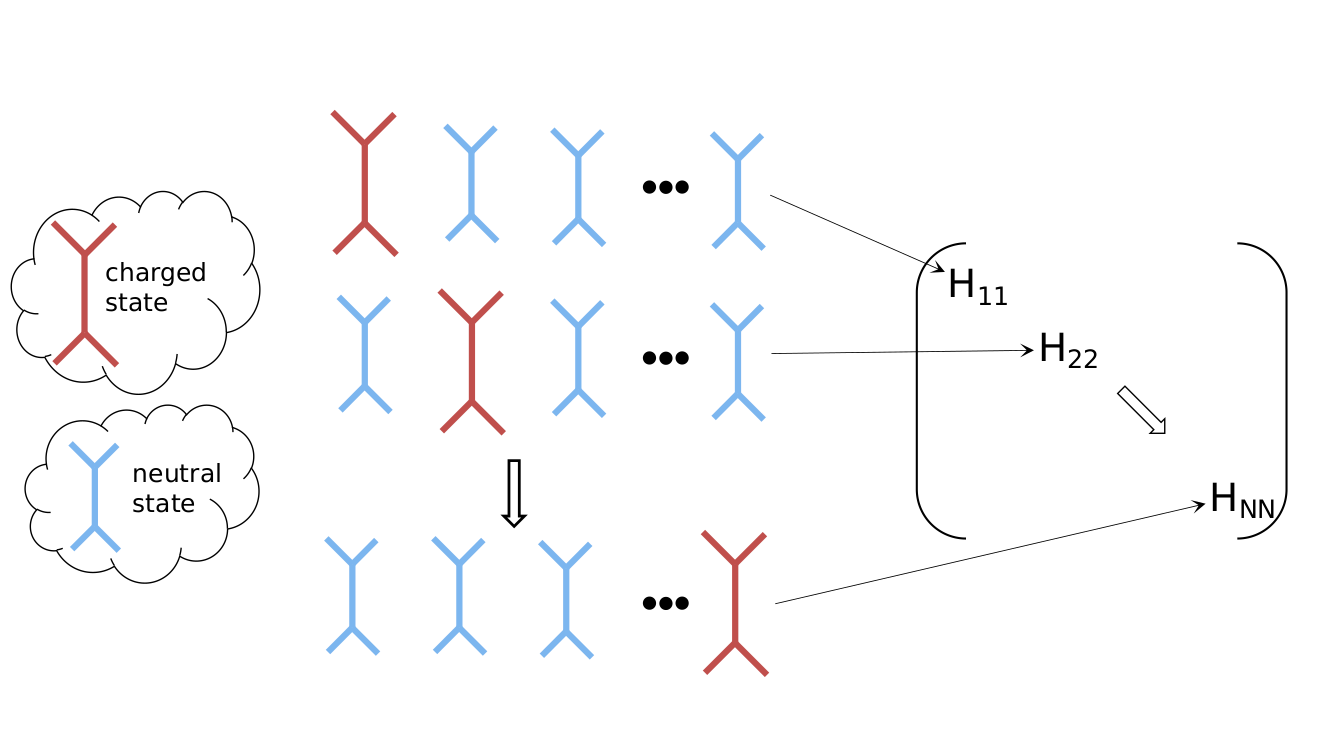
\includegraphics[width=\textwidth]{../img/ES/ForceEnerCalc.png}
  \caption{\label{fig:FE_Calc}A demonstration of the procedure to calculate diagonal elements of the Hamiltonian (site-energies). Red (blue) shapes represent a molecule in its charged (neutral) state. A  horizontal line of these shapes represent the full system with all molecules; where a single molecule is in its charged state. The arrow denotes which matrix element this saved as.}
\end{figure}
\noindent In FOB-SH, the electronic Hamiltonian is constructed such that the diagonal elements (site-energies) come from a classical forcefield and the off-diagonal elements (electron couplings) are estimated using the ultrafast atomic overlap method(AOM). These are proportional to the overlap of the diabatic wavefunctions. Each site-energy, $H_{\gamma \gamma}$, is defined as the potential energy of the system where the excess charge is localised on the molecule $\gamma$. For the avoidance of doubt, I will denote the molecule with the excess charge localised on it as the `charged' molecule and other molecules as `neutral'. The presence of the excess charge on molecule $\gamma$ results in different input parameters (such as the charge distribution or the length of bonds) than the other neutral molecules. This results in the calculation of site-energies and forces having to be repeated $N_{mol}$ times for each permutation of the charged molecule. This is summarised in figure \ref{fig:FE_Calc}. 
\\\\
To determine whether it is feasible to repeat the calculation of the electrostatic interactions $N_{mol}$ times a quick timing run was carried out. This simulated two hundred and fifty pentacene molecules (nine thousand atoms) and the time was measured to calculate the electrostatic interactions with the three methods already implemented within CP2K: Smooth Particle Mesh Ewald (SPME), Particle Mesh Ewald (PME) and standard Ewald. The measured time of a simulation without any electrostatics was then subtracted from each of these simulations to isolate the time spent on just the electrostatics. The results are given in figure  \ref{fig:ES_Timings}.
\begin{figure}[ht]
  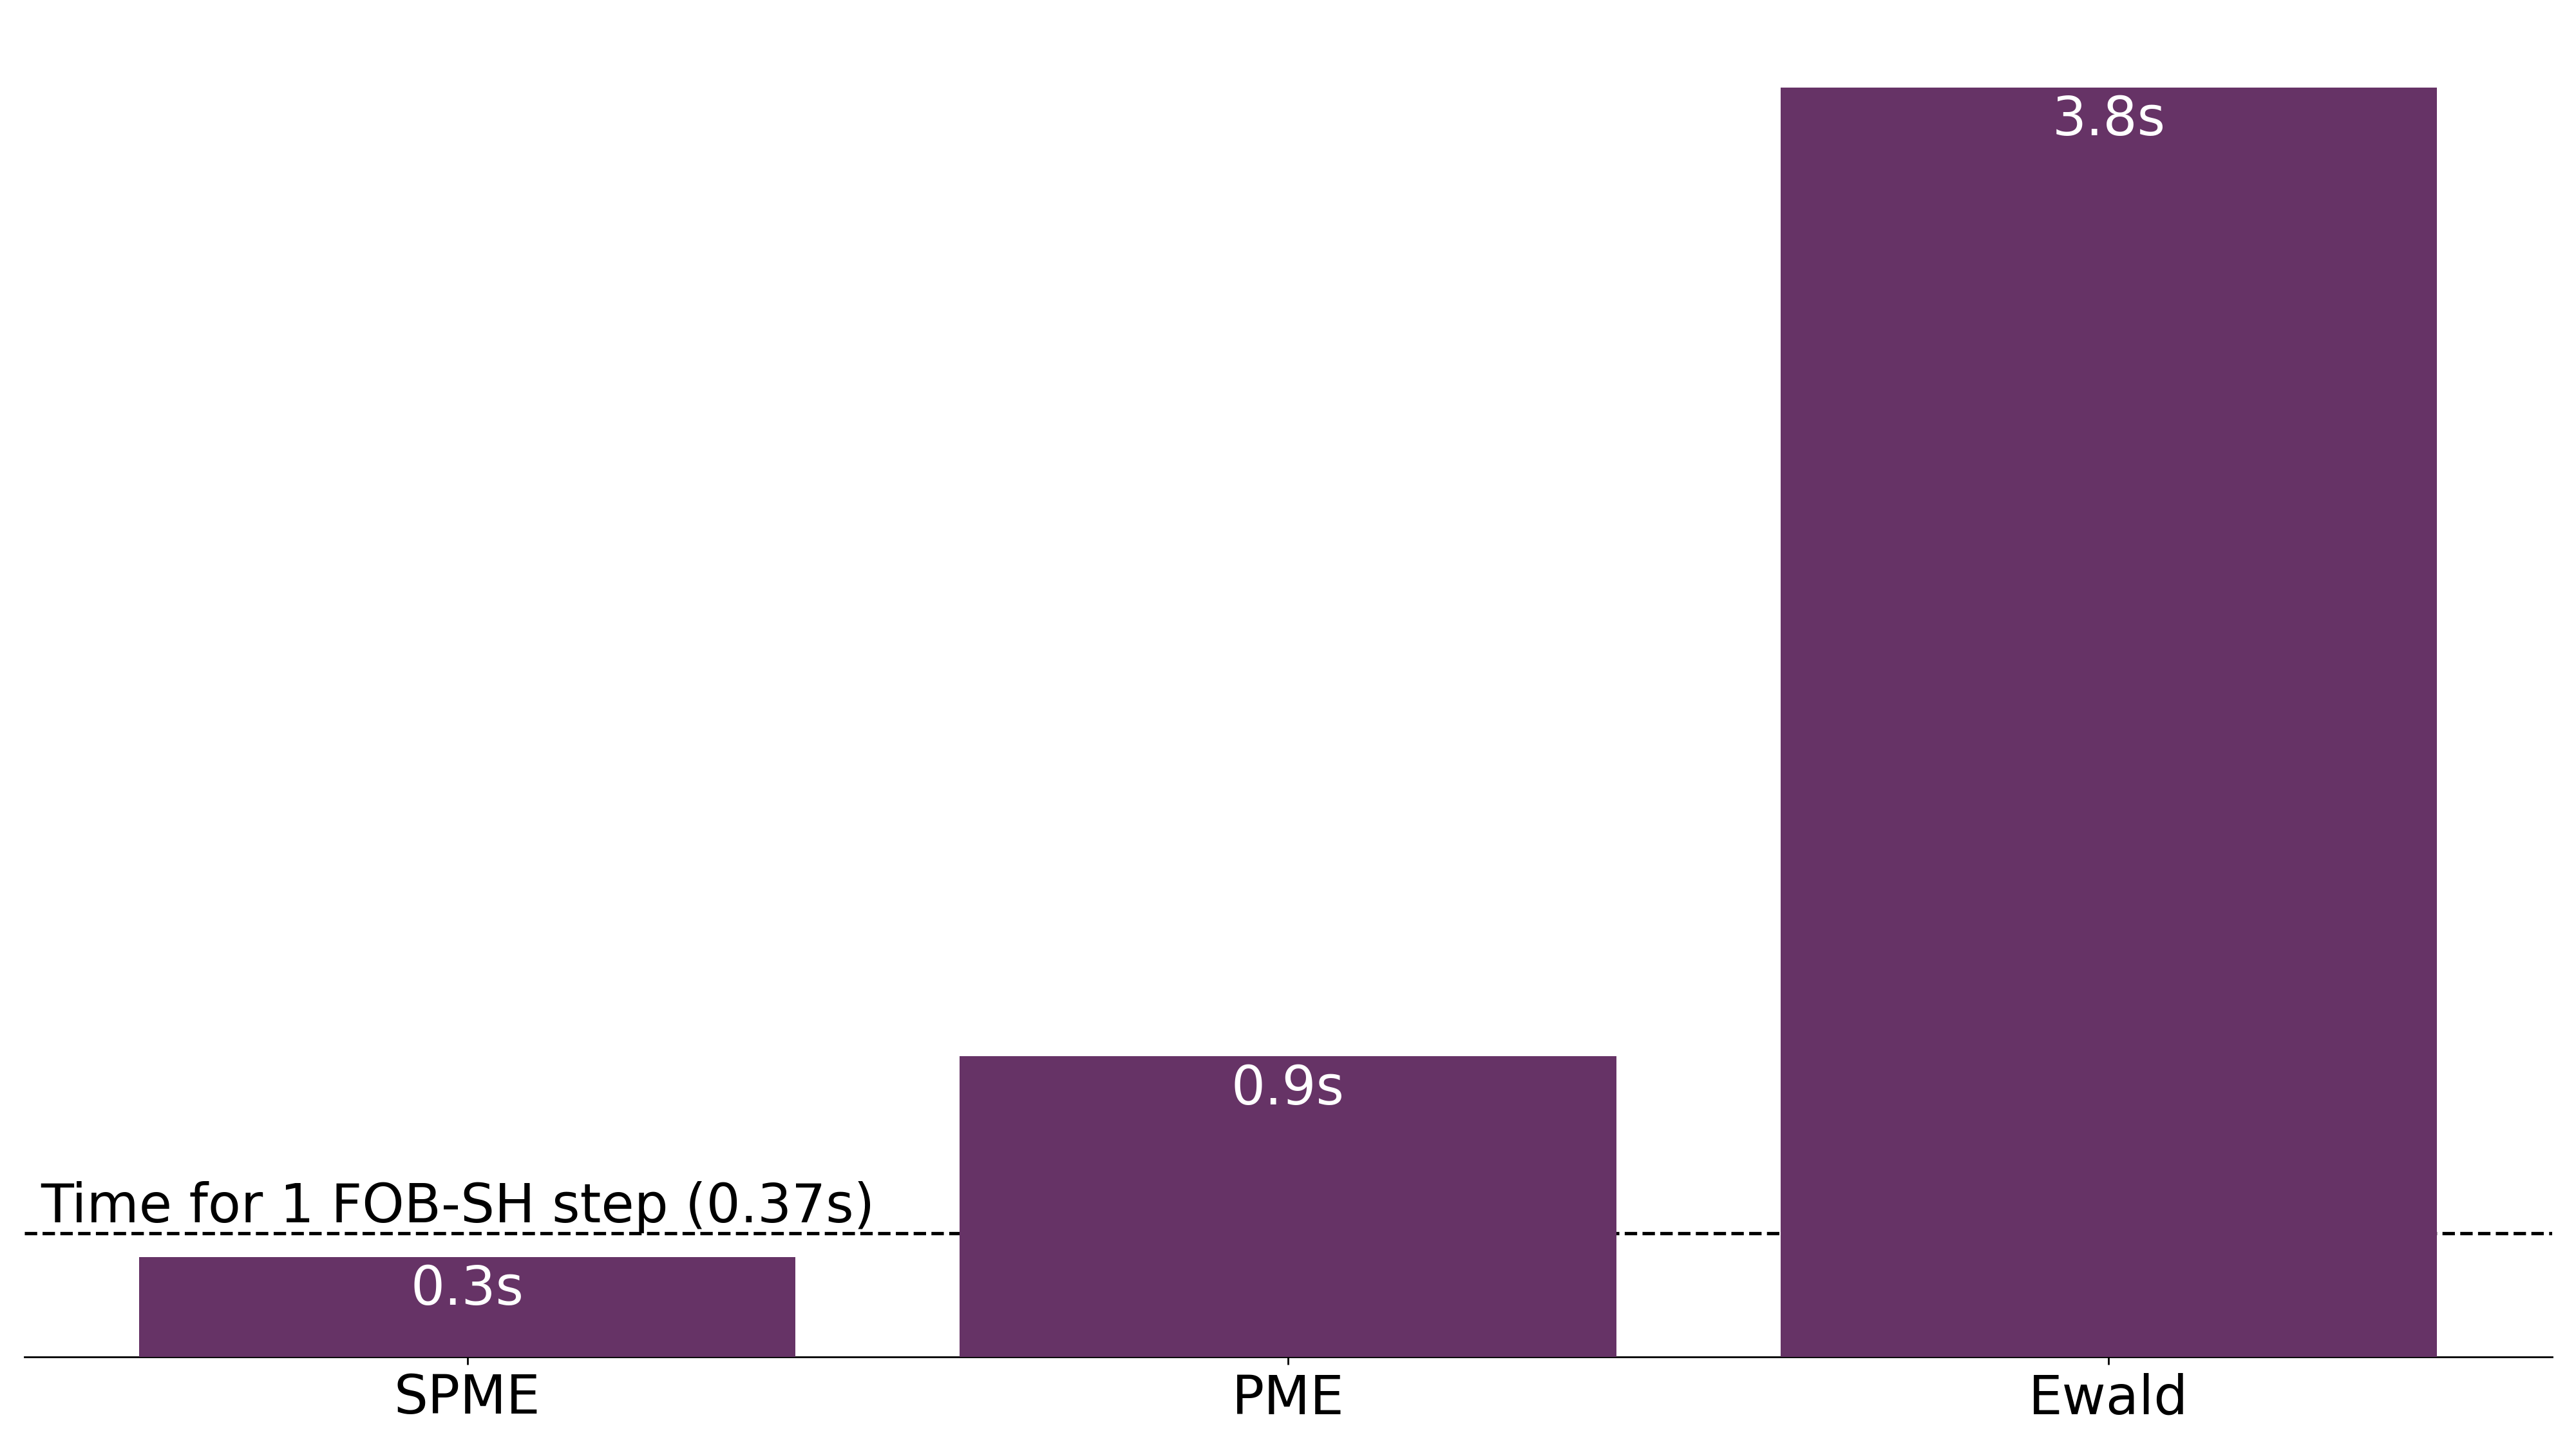
\includegraphics[width=\textwidth]{../img/ES/InitialTimings.png}
	\caption{\label{fig:ES_Timings}The time taken to calculate just the electrostatic interactions within CP2K for a nine thousand atom system using various methods. PME is particle mesh Ewald, SPME is smooth-PME, Ewald is the standard ewald method. The dashed line shows the time taken for a single FOB-SH step.}
\end{figure}
\\
We can see that even a single calculation of the electrostatic interactions with the fastest method available within CP2K (SPME) will take a length of time comparable to the rest of the surface hopping code. It is clear then that a more efficient method must be used to calculate the electrostatics.
\\
\begin{figure}[ht]
  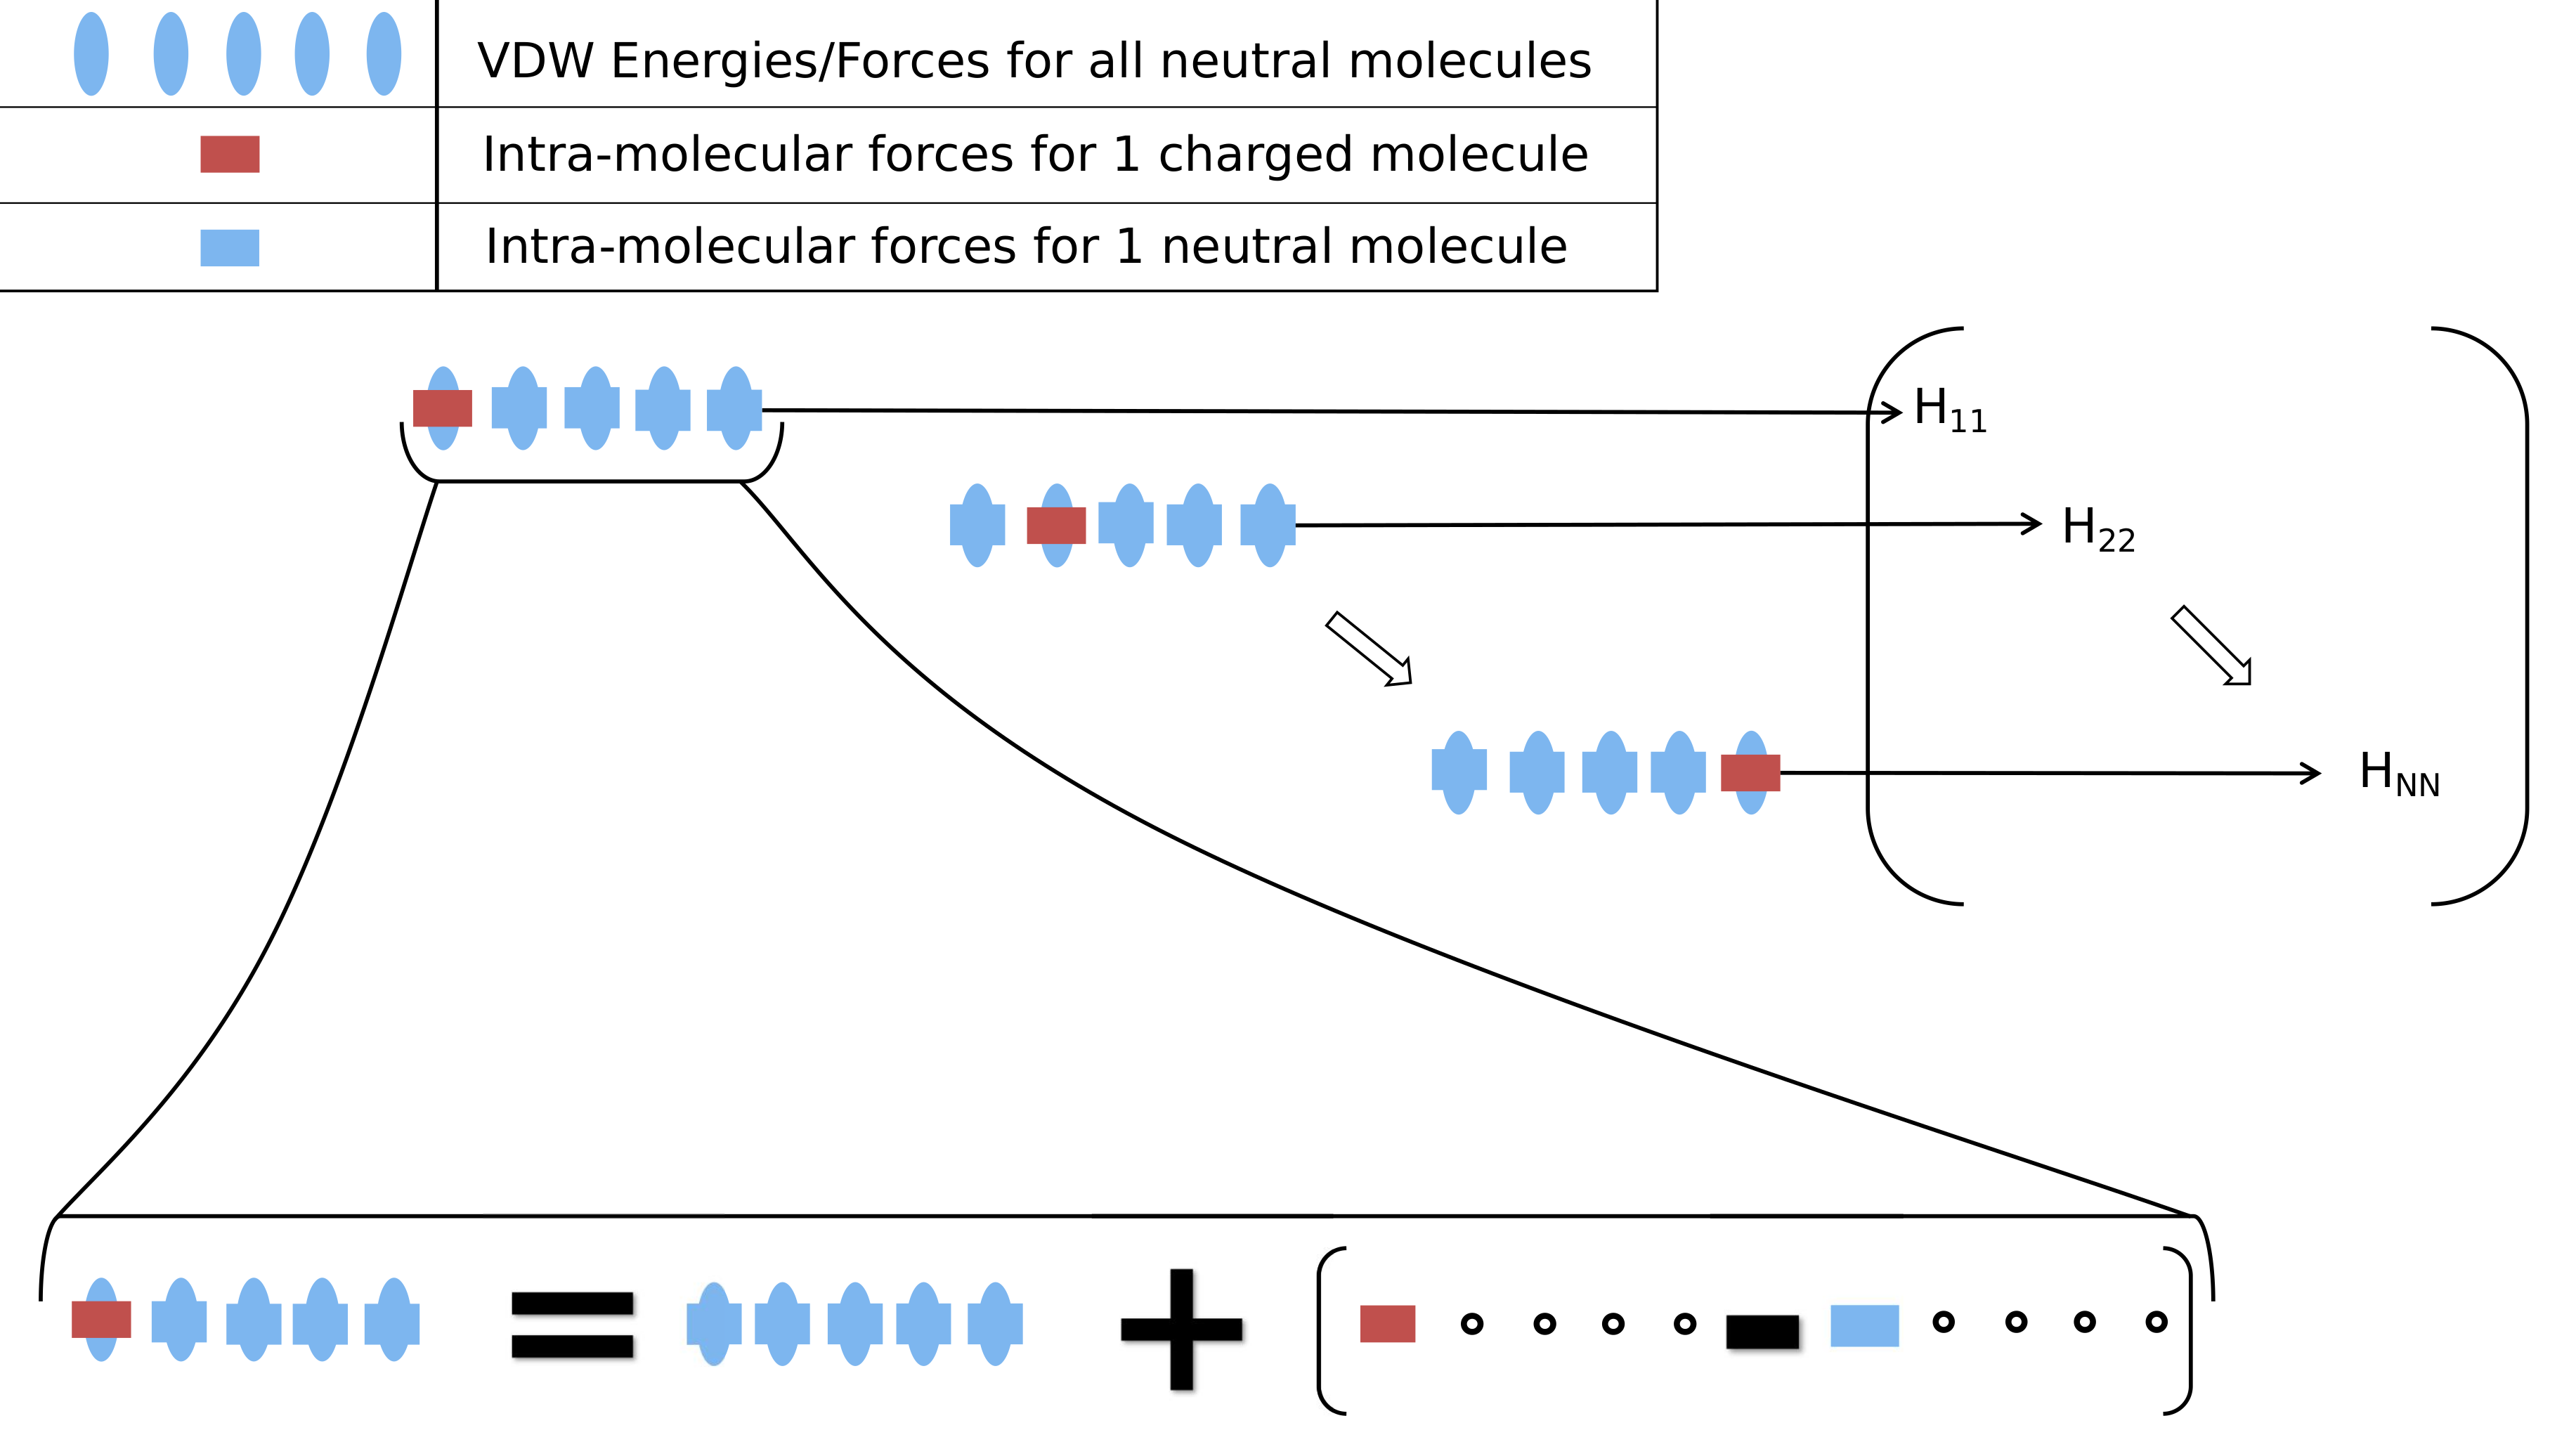
\includegraphics[width=\textwidth]{../img/ES/ForceEnerDecomp.png}
  \caption{\label{fig:enerF_decomp}A depiction of the decomposition of the forces and energies within FOB-SH. First the all neutral VDW forces/energies are computed (blue ovals). Second the intra-molecular forces for each charged (neutral) molecule, represented by a red (blue) rectangle. The site-energy/force is then computed as a summation of all molecules in their neutral state with a molecule in its neutral state subtracted and the same molecule in its charged state added.} 
\end{figure}
\\
To calculate the intramolecular and Van der Waals energies and forces within the current FOB-SH implementation, the forces and energies consist of intra-molecular components (bonds, bends, torsions etc\ldots) and inter-molecular components (Van der Waals forces provided by a Leonard-Jones potential). The same repetition of the calculation of forces and energies would, at first glance, be required for the correct calculation of these terms. However, an addition-subtraction scheme is used to reduce the calculation time from $O(N_{mol} N_{atom}^2)$ to $O(N_{atom}^2)$. This is summarised in figure \ref{fig:enerF_decomp} and relies on the fact that the intra-molecular forces and energies can be decomposed into independent molecular contributions. In order to calculate the force on each atom and site-energy with molecule $\gamma$ in its charged state the code first calculates the force/energy with all molecules in their neutral state and then adds the contribution of molecule $\gamma$ in its charged state and subtracts the contribution of molecule $\gamma$ in its neutral state. We do not make the same adjustment for the VDW forces as the difference is exactly zero if one assumes that VDW does not depend on the charge state (which is customary in force fields). This results in just two calculations of all forces and total energies rather than $O(N_{mol})$ calculations. This scheme can be used because the intra-molecular forces can be naturally decomposed into discrete molecular contributions. That is, the calculation of the intra-molecular interactions are decoupled from their environment are independent of the charge state of all other molecules. The electrostatic interactions are, unfortunately, not so intuitively broken down. However, a similar trick can be used to reduce the cost of the Ewald sum. In the following work, I will present two frameworks in which to calculate electrostatic interactions: the recalculation method and the addition-subtraction method. The recalculation method references the method of na\"ively looping over all molecules and recalculating energies and forces without optimisations. This would involve recalculating all interactions for every permutation of charged/neutral molecules. The addition-subtraction scheme is explained in the proceeding chapters.
\subsection{Ewald Equations and the additional subtraction scheme}
The standard Ewald summation for evaluating electrostatic energies in molecular dynamics simulation are given below:
\begin{align}
  \begin{split}
E_{coul}\left(\mathbf{r}\right)
=
% Real Space Sum
	  \frac{1}{4 \pi \epsilon_0} \sum_{\mathbf{n}} \ ^{'} \sum_{j}^{N_{at}^{*}} \sum_{i \neq j}^{N_{at}^{*}} q_i q_j \frac{erfc\left( \alpha \cdot |\mathbf{r}_{ij} + \mathbf{n}|\right)}{|\mathbf{r}_{ij} + \mathbf{n}|} \Theta\left( r_{cut} - |\mathbf{r}_{ij} + \mathbf{n}| \right)
\\
% Reciprocal Space Sum
+
\frac{4 \pi}{ V} \ \sum_{\mathbf{k} \neq 0} \frac{1}{|\mathbf{k}|^2} e^{-\frac{\pi^2 \ |\mathbf{k}|^2}{\alpha^2}} \ \left|\sum_{j}^{N_{at}} q_{j} e^{2\pi i \mathbf{k} \cdot \mathbf{R}_{j}}\right|^2 \\
% Self Term
- \frac{\alpha}{\sqrt{\pi}} \sum_{j} q_{j}^2
\\
% Bonded Correction Term
	  - \sum_{(i,j) \in (\text{1-Z list)}}\left(E^{1-2}_{ij} + E^{1-3}_{ij} + (1 - \zeta)E_{ij}^{1-4} \right)
	\end{split}
\label{eq:EwaldStd}
\end{align}
In equation \eqref{eq:EwaldStd}, the first term is the real space sum. This sums over all periodic images ($\mathbf{n}$) and pairs of atoms $i$, $j$ within a cutoff imposed by the Heaviside step function $\Theta(r_{cut} - |\mathbf{r}_{ij}+\mathbf{n}|)$. The relative position vector between atoms is given by $\mathbf{r}_{ij} = \mathbf{r}_{i} - \mathbf{r}_{j}$, the charge on atom $i$ is given by $q_{i}$ and alpha is a convergence parameter. The $^{*}$ symbol highlights that the loop should be over all non-bonded atoms. The second term is the most expensive part of this calculation and sums over reciprocal space vectors $\mathbf{k}$ and atoms, $j$. $\mathbf{R}_{j}$ represents the position vector of atom $j$. The third term is the constant self-energy term and the fourth corrects for bonded (intra-molecular) interactions. In the bonded correction $E_{ij}^{1-Z} = \frac{1}{4 \pi \epsilon_{0}} q_{i}q_{j} \frac{erf\left( \alpha \cdot |\mathbf{r}_{ij} + \mathbf{n}|\right)}{|\mathbf{r}_{ij} + \mathbf{n}|}$. This removes the contribution of bonded interactions, which are accounted for by the intramolecular forcefield. These interactions are easily removed from the first term (real space sum) by simply not looping over the atoms, so this correction acts to amend the energy from the reciprocal space sum.
\\\\
As these four summations are independent we can look at each one separately when implementing the addition-subtraction scheme, starting with the simplest, the self-energy term. Note in this section I will only discuss the energies; the forces are very similar and their equations are given in appendix \ref{ap:EwaldForcesAddSub}.
\subsection{Self-energy addition subtraction scheme}
The self energy term is a correction for over counting within the reciprocal space sum. For each site-energy, $\gamma$, we must recalculate the full forces and energies with the excess charge located on molecule $\gamma$. This is demonstrated in equation \eqref{eq:SelfNoScheme}. Note that for brevity I have replaced the factor $\frac{1}{4 \pi \epsilon_0}$ with $\eta$.
\begin{equation}
  E_{self}^{\gamma} = \frac{\alpha}{\sqrt{\pi}} \eta \left[\sum_{j \not\in \gamma} \left(q^{n}_{j}\right)^2  + \sum_{j \in \gamma} \left(q^{c}_{j}\right)^2\right]
  \label{eq:SelfNoScheme}
\end{equation}
In the above equation, the Ewald self-energy correction contribution for site-energy $\gamma$ is simply a sum of squared neutral state charges for atoms belonging to molecules that aren't $\gamma$ plus the sum of squared charged state charges of atoms within $\gamma$. For clarity, the terms `neutral state charges' and `charged state charges' refer to charges with molecules parameterised in their neutral (no excess charge carrier) and charged (excess charge carrier localised on the molecule) state. This is represented by the superscript $n$ and $c$ where $q^{n}_{j}$ represents the charge on atom $j$ where the force-field for the molecule it belongs to has been parameterised in its neutral state. $q^{c}_{j}$ represents the charge on atom $j$, where the force-field for the molecule the atom belongs to has been parameterised in its charged state.
\\\\
For a single molecular type system, this value is the same for all $\gamma$ and no optimisations are required, except to calculate this value once and use it for each $\gamma$. However, for a more complex system the addition subtraction scheme used is given in equation \eqref{eq:SelfScheme}.
\begin{equation}
  E_{self}^{\gamma} = \eta \underbrace{\frac{\alpha}{\sqrt{\pi}} \sum_{j}^{N_{at}}\left(q_{j}^{n}\right)^2}_{\text{Calculated Once}} + \underbrace{\frac{\alpha}{\sqrt{\pi}} \eta \sum_{j \in \gamma} \left[ (q^{c}_{j})^2 - (q^{n}_{j})^2 \right]}_{\text{Calculated for each $\gamma$}}
  \label{eq:SelfScheme}
\end{equation}
In equation \eqref{eq:SelfScheme} we have removed the $\gamma$ index from the most expensive part of the sum; this means we can calculate it once and store it. In the second term we only sum over atoms in charged molecule $\gamma$ and remove the contribution from molecule $\gamma$ in its neutral state and add the contribution from molecule $\gamma$ in its charged state. Seeing as the correction part of equation \eqref{eq:SelfScheme} is the only part repeated from each $\gamma$ this reduces the cost of this calculation from $O(N_{mol}, N_{atom})$ to just $O(N_{atom})$. The same idea is used for the remaining terms in the Ewald sum.
\subsection{Real space addition subtraction}
The real space term is more complicated than the self-energy term, though the idea is the same. That is, the fully neutral contribution is calculated and for individual sites/molecules a correction is applied. This is shown in equation \eqref{eq:RealScheme}
\begin{align}
  \begin{split}
	  E^{\gamma}_{real} &= \eta \sum_{\mathbf{n}} \sum_{j}^{N_{at}} \sum_{i}^{N_{at}} q^{n}_i q^{n}_j  \ R^{dir}(|\mathbf{r}_{ij} + \mathbf{n}|) \\
	  &+ \eta \sum_{\mathbf{n}} \sum_{j \in \gamma, i \in \gamma} (q_j^c q_i^c - q_j^n q_i^n) \ R^{dir}(|\mathbf{r}_{ij} + \mathbf{n}|) \\
	  &+ \eta \sum_{\mathbf{n}} \sum_{j \in \gamma, i \not\in \gamma} (q_j^c - q_j^n)q_i^n \ R^{dir}(|\mathbf{r}_{ij} + \mathbf{n}|) 
  \end{split}
  \label{eq:RealScheme}
\end{align}
In equation \eqref{eq:RealScheme} the most expensive summation ($O(N_{atom}^2)$) is the first term. Fortunately, we can once again calculate this once and use the same value for each site-energy. This first term calculates all interactions between atoms belonging to molecules in their neutral state (interactions between molecules both in their neutral state). The next two terms show the addition-subtraction correction. The second term shows a sum over all pairs of atoms in the charged molecule, $\gamma$. In this term we subtract any interactions with both molecules in their neutral state and replace them with any charged-charged interactions. This scales as $O(N_{\text{atom per mol}})$ and is repeated $N_{mol}$ times so the full correction scales as $O(N_{atom})$. The third term replaces any interactions of atoms on the charged molecule with its environment (neutral molecules), hence it removes neutral-neutral interactions and replaces them with charged-neutral interactions. This scales as $O(N_{\text{atom per mol}}, N_{atom})$ and is repeated $N_{mol}$ times, resulting in an ultimate scaling of $O(N_{atom}^2)$. Therefore, this optimisation scales in the same manner as a single calculation of the Ewald interactions and any additional overheads will be minimal. For the avoidance of doubt, in equation \eqref{eq:RealScheme} I have replaced the complementary error function and Heaviside step function in equation \eqref{eq:EwaldStd} with the term $R^{dir}(|\mathbf{r} + \mathbf{n}|)$, i.e. $R^{dir}(|\mathbf{r}_{ij} + \mathbf{n}|) = \frac{erfc\left( \alpha \cdot |\mathbf{r}_{ij} + \mathbf{n}|\right)}{|\mathbf{r}_{ij} + \mathbf{n}|}              \Theta\left( r_{cut} - |\mathbf{r}_{ij} + \mathbf{n}| \right)$

\subsection{Bonded corrections addition subtraction}
The bonded correction terms remove electrostatic contributions to energies (and forces) for atoms that are bonded. This is because interactions are already accounted for by the intra-molecular force-field (bonds, bends, torsions etc\ldots). These interactions occur within molecules and their contribution can be decomposed into molecular contributions. These interactions can therefore be handled in the same way as the intra-molecular addition-subtraction scheme as discussed in section \ref{sect:addSubMethod}. The correction is given in equation \eqref{eq:EwaldStd} and just involves looping over atoms that are bonded and subtracting the coulomb energy and forces from the total.

\subsection{Reciprocal space addition subtraction}
The correction for the reciprocal space sum is given below in equation \eqref{eq:RecipScheme}.
\begin{equation}
  E^{\gamma}_{recip} = \frac{1}{2 \pi V} \sum_{\mathbf{k} \neq 0} \frac{1}{|\mathbf{k}|^2} e^{\frac{\pi^2 |\mathbf{k}|^2}{\eta^2}} \left| \sum_{j}^{N_{at}} q^{n}_{j} e^{2 \pi \mathbf{k} \cdot \mathbf{R}_{j}}  + \sum_{j \in \gamma}^{N_{at}} (q^{c}_{j} - q^n_j) e^{2 \pi \mathbf{k} \cdot \mathbf{R}_{j}} \right| ^2
  \label{eq:RecipScheme}
\end{equation}
The idea here is the same. The first term, looping over all neutral state charges, is calculated just once. The second term is then repeated for every state/molecule. This corrects term one which only includes interactions of neutral state molecules with neutral state molecules. This is done by adding the charged state contribution and subtracting the neutral state contribution.
\\\\
The reciprocal energies can be optimised using the addition-subtraction technique. However, the forces cannot. I have given the equation for the forces below in \eqref{eq:AddSubForcesRecip}
\begin{equation}
    \F_{i}^{\gamma}(\mathbf{R}) =  \left\lbrace \begin{array}{lc}
      4\pi q_{i}^{C} \sum_{\mathbf{k} \neq 0} \mathrm{Im}\left[ S^{'}_{\mathbf{k}} E_{\mathbf{k},i}^{*} \right]; & i  \in \gamma\\\\
    
    4\pi q_{i}^{N} \sum_{\mathbf{k} \neq 0} \mathrm{Im}\left[ S^{'}_{\mathbf{k}} E_{\mathbf{k},i}^{*} \right];& i     \notin \gamma
    \end{array}
    \right.
    \label{eq:AddSubForcesRecip}
\end{equation}
Where:
\begin{itemize}
  \item $S_{\mathbf{k}}^{'} = A_{\mathbf{k}} \left[\sum_{j} q_j^{N} E_{\mathbf{k}, j} + \sum_{j \in \gamma}           \left(q_j^{C} - q_{j}^{N}\right) E_{\mathbf{k}, j}\right]$

  \item $A_{\mathbf{k}} = \frac{\mathbf{k}}{|\mathbf{k}|^2} e^{\frac{|\mathbf{k}|^2}{4 \alpha^2}}$

  \item $E_{\mathbf{k}, j} = e^{2 \pi \mathrm{i} \mathbf{k} \cdot \R_{j}}$
\end{itemize}
\noindent The calculation of this equation scales as $\mathcal{O}(N^3)$ where $N^3 = N_{states} N_{atom} N_{k}$. This   is because for every atom, $i$, in charged molecule, $\gamma$, a loop over $\mathbf{k}$ vectors must be calculated.   
\\\\
This is a big problem for any implementation of Ewald electrostatics within surface hopping as the reciprocal space part of the Ewald sum is by far the most expensive part of the electrostatics calculation. In fact in the same two hundred and fifty molecule system as in figure \ref{fig:ES_Timings} the reciprocal space component took eighty eight percent of the calculation time. In larger systems this increases. Repeating this calculation $N_{mol}$ times would be far too slow and would limit the surface hopping code to small systems of tens of molecules. However, the damped shifted forces technique (DSF) \cite{DSF} can be used to approximate the electrostatic interactions without the reciprocal force term. 
\section{Timing the electrostatics implementation}
\begin{figure}[ht]
  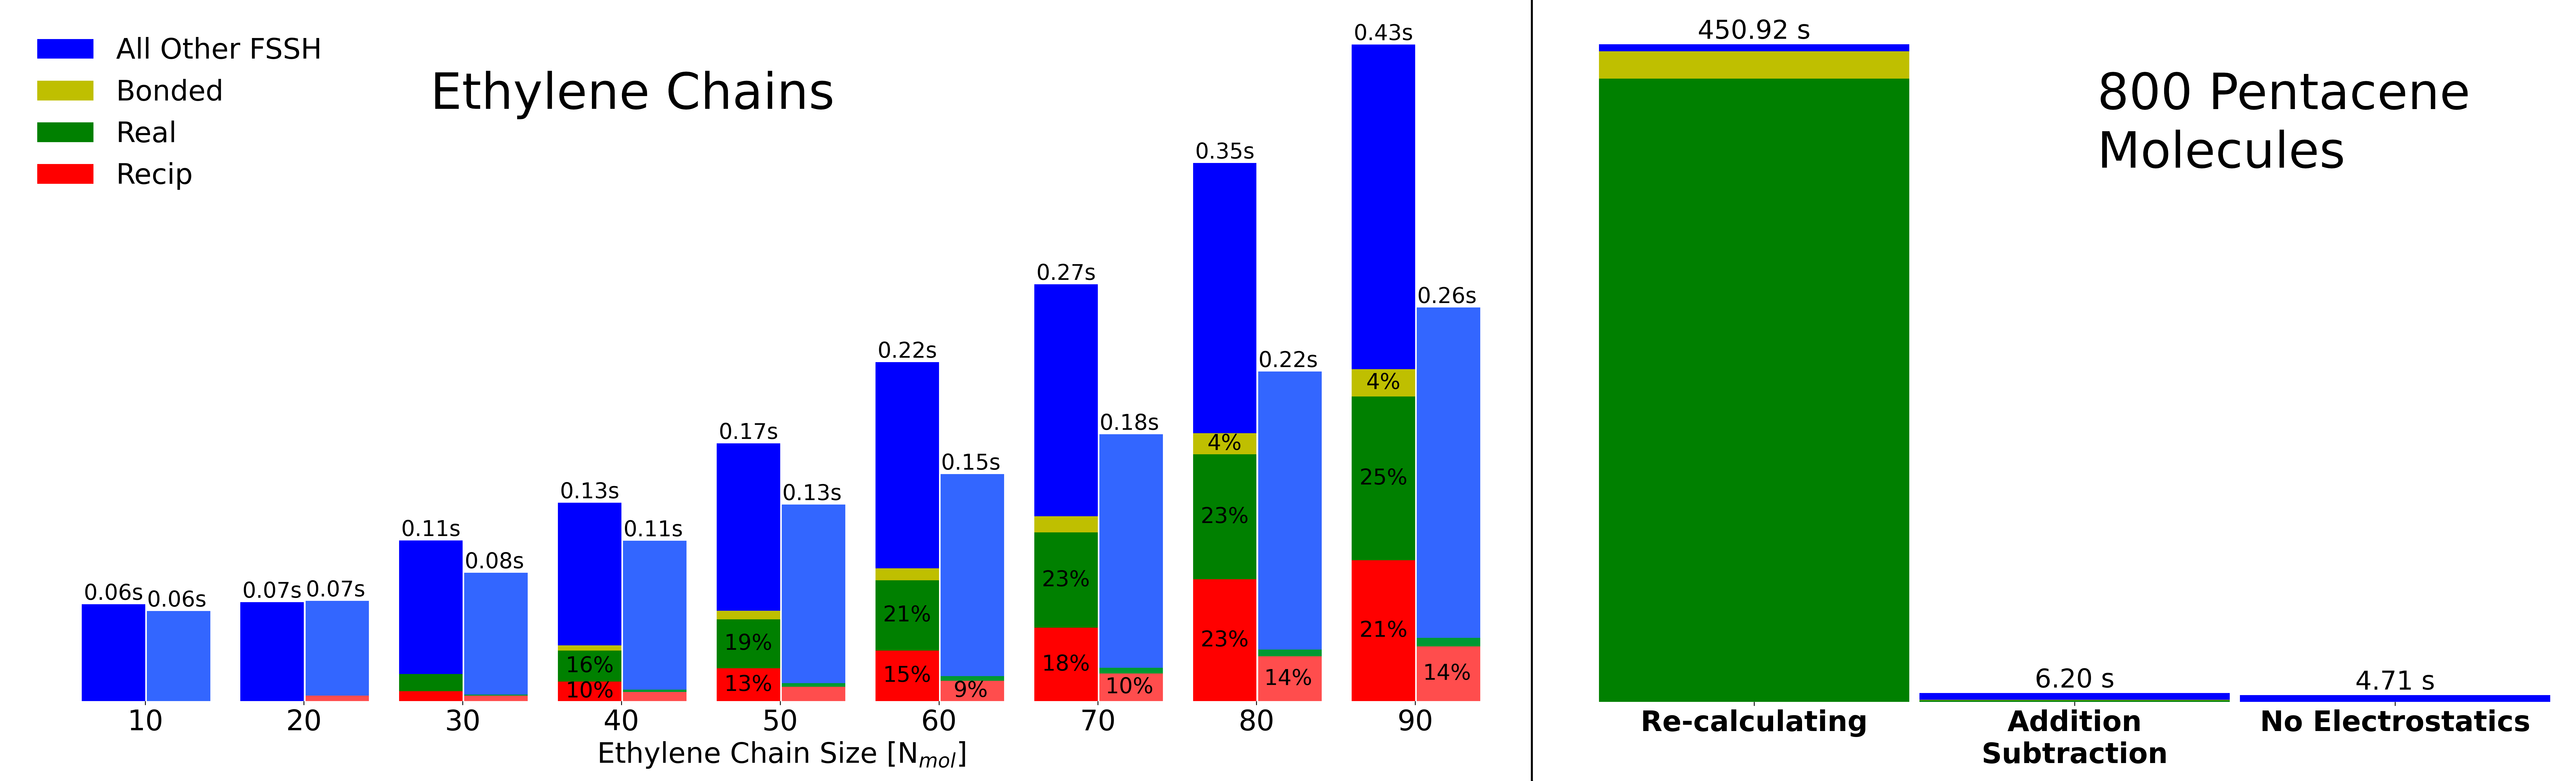
\includegraphics[width=\textwidth]{../img/ES/TimingsReCalc_vs_AddSub.png}
	\caption{\label{fig:AddSubTimings}Time taken to run surface hopping and electrostatics for various lengths of one dimensional ethylene chain (left) and eight hundred molecule pentacene plane (right). Darker colors show data from the recalculation method for the electrostatics and less saturated colors to the right show data from the addition subtraction scheme. Green bars show the time taken to calculate real space interactions, red is reciprocal, yellow is the bonded corrections and blue shows all other parts of the surface hopping code. In the right pane reciprocal interactions are omitted as they took too long to run.}
\end{figure}
\noindent In figure \ref{fig:AddSubTimings} the time taken for a single step of a surface hopping simulation for various lengths of a one dimensional ethylene chain can be seen (left panel). We see as the chain size increases it becomes more important that electrostatic interactions are efficiently handled. In fact for just a ninty molecule ethylene chain calculating the electrostatics takes longer than all other parts of surface hopping. On the right of the same figure, timings for a eight hundred molecule pentacene plane are shown. In these simulations, the reciprocal calculations took far too long and had to be turned off to measure the time taken for the other components. In this panel we see the significant speed-up for larger system sizes when using the addition-subtraction scheme. However, even with the addition-subtraction scheme the full reciprocal space calculations still take far too long. This is because the calculation of the forces are still repeated $N_{mol}$ times as they cannot be optimised in the same way. A small speedup is seen due to the addition-subtraction scheme being used with the reciprocal space energies. However, we see that the addition-subtraction scheme offers a major speedup for all other components. It is, of course, also vital that the results outputted are correct. I have tested both the recalculation method and the addition-subtraction method against standard CP2K calculations to ensure the implementation is correct. In the following section I will present results only for the addition-subtraction scheme although the re-calculation method was tested in the same way.


\subsection{Testing the electrostatics implementation}
\label{sect:testESimp}
To test the calculation of site-energies and forces within CP2K a ten molecule ethylene chain was used. In order to produce reference data the new implementation could be checked against, classical MD in CP2K was used to calculate the site-energies and forces for ten different system. In each one of these simulations a different molecule was chosen to have charged geometry and the rest were chosen to have neutral geometry in the input files. A single step of MD was then carried out and forces and energies were outputted. These forces and energies were subsequently compared to the forces and energies outputted by the both the recalculation and addition-subtraction method. The results for the tests of the addition-subtraction method are shown in figure \ref{fig:AddSubEwaldTest}.
\begin{figure}[ht]
  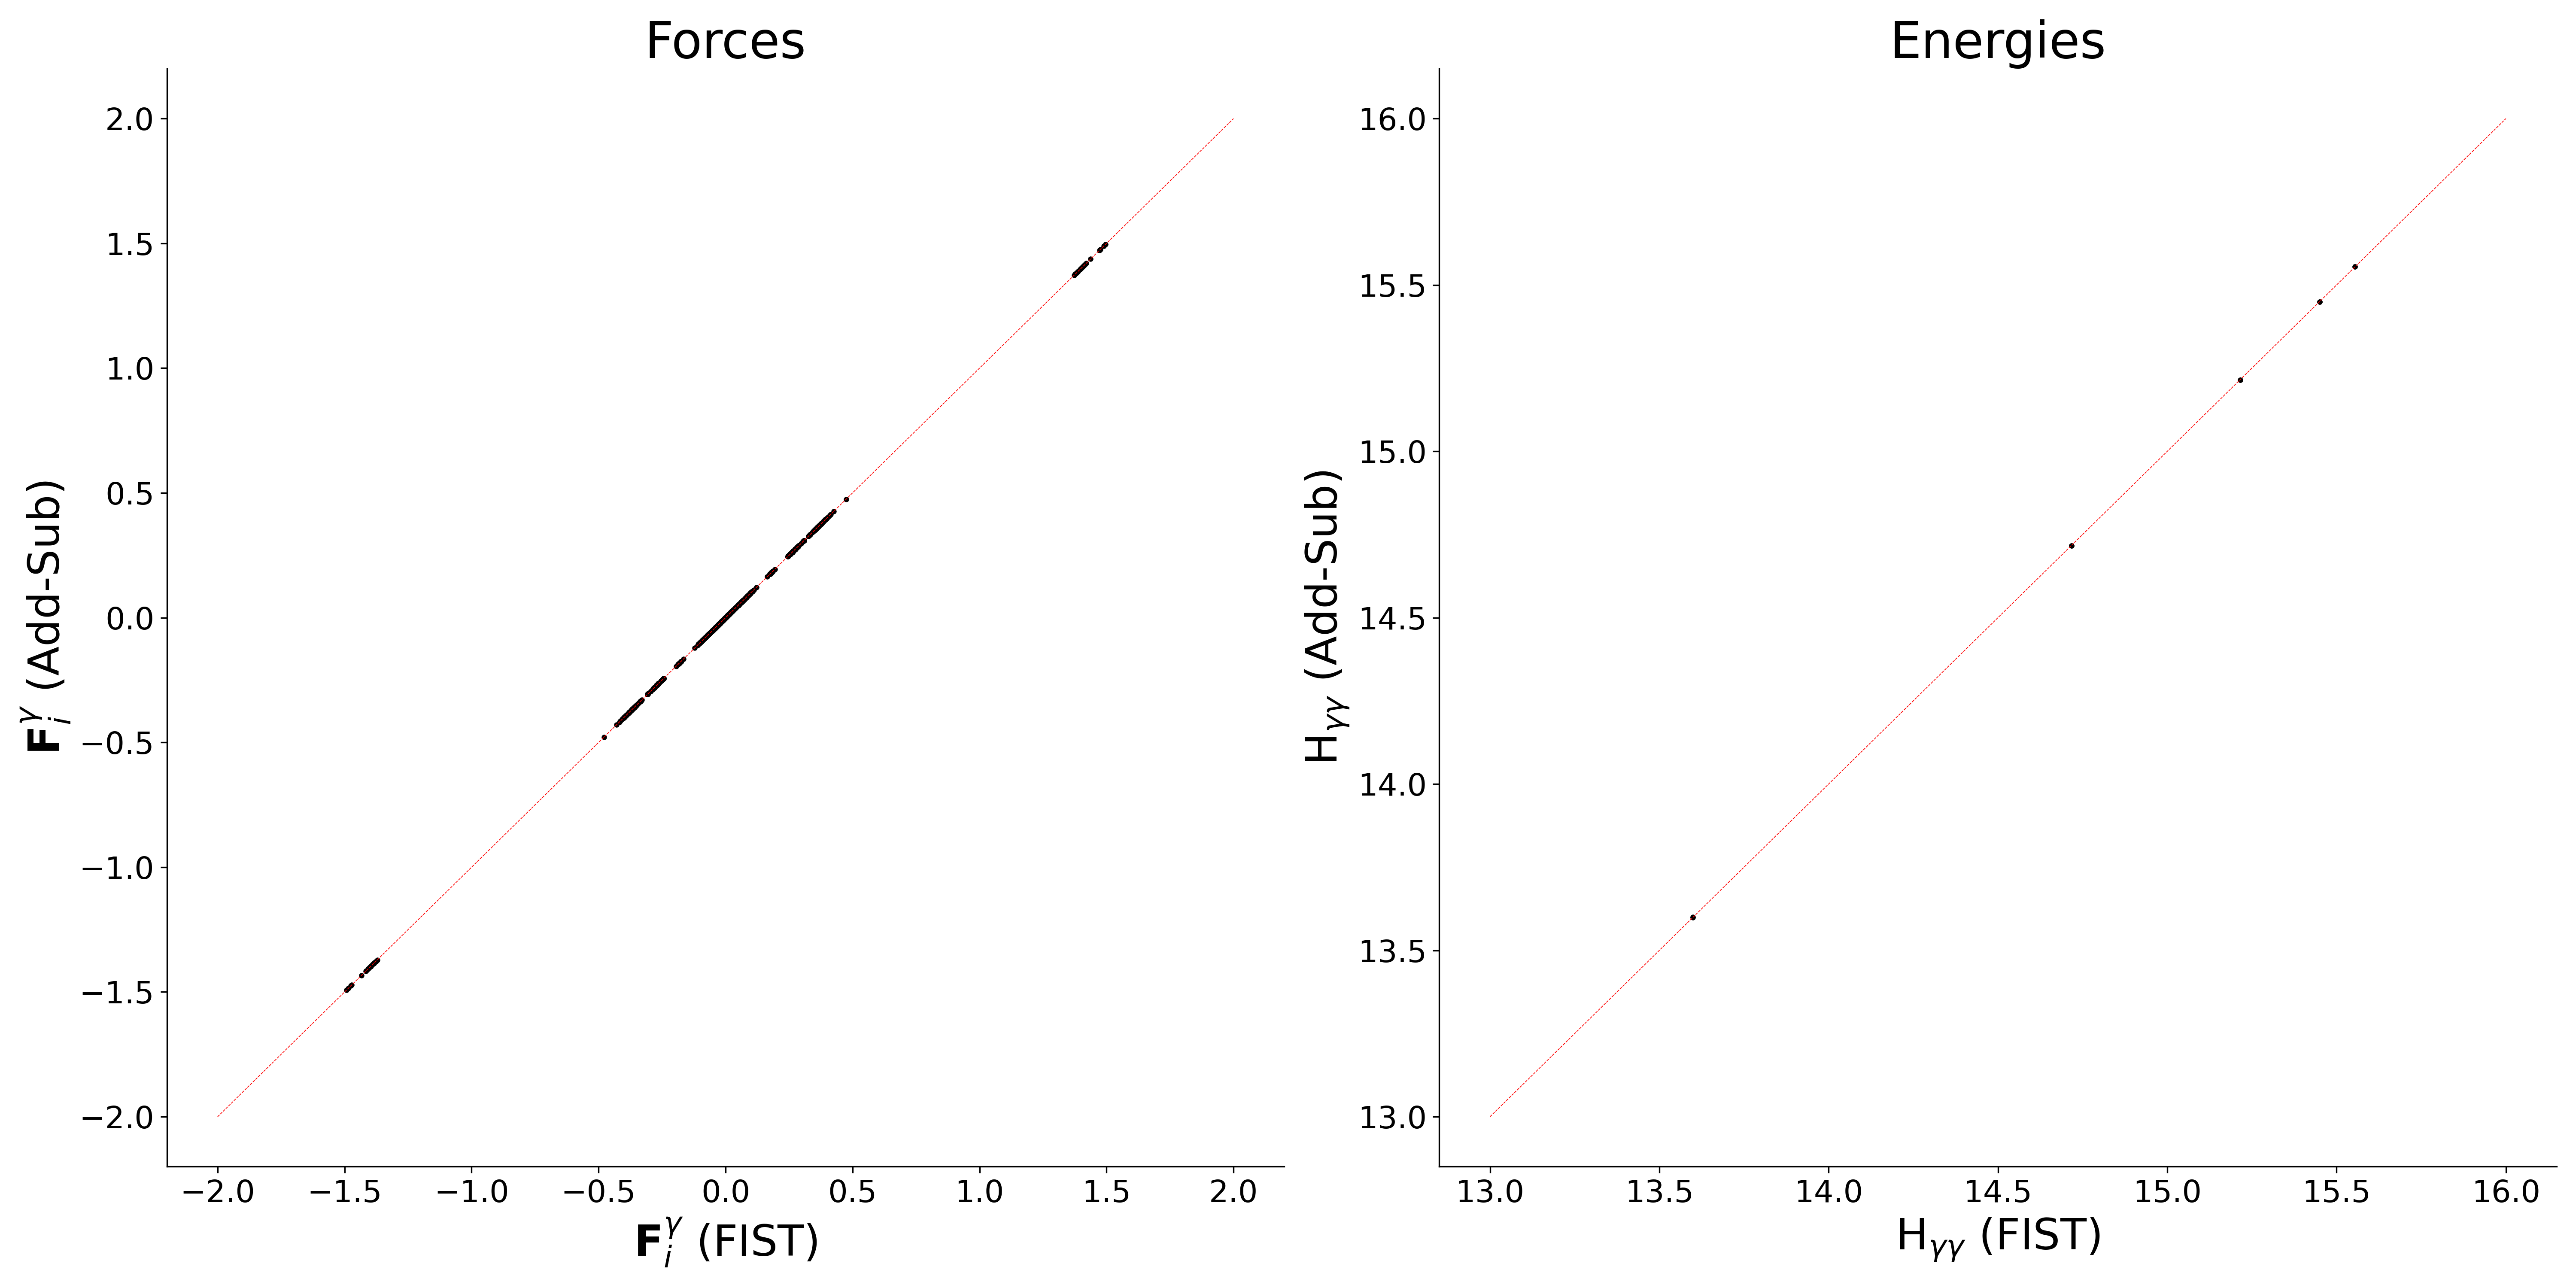
\includegraphics[width=\textwidth]{../img/ES/10_mol_FIST.png}
	\caption{\label{fig:AddSubEwaldTest}A comparison of forces and energies calculated with multiple classical MD simulations (x-axis) and the addition-subtraction method with Ewald electrostatics. The left pane shows the magnitude of the outputted forces and the right the outputted potential energies. Black dots show values from each atom and timestep. The red dashed line shows $y=x$ and serves as a guide for the eye.}
\end{figure}
We see in figure \ref{fig:AddSubEwaldTest} that the values of energy and forces as calculated with CP2K's standard MD package (FIST) and my implementation of the addition-subtraction method are exactly the same. In fact the maximum absolute difference between results was 5$\times 10^{-13}$ i.e. numerical noise. This confirms the implementation of the addition-subtraction scheme. It should be noted that the values for the forces and energies are rather large. This is due to the ethylene system used not being equilibrated. The system was created by placing ten ethylene molecules in a line with a two Angstrom spacing. As this test wasn't a test of the physics of the system but the implementation of the equations it does not matter that the system was quite unphysical.
\\\\
To further benchmark the addition-subtraction scheme the same input parameters were fed into the code using the recalculation method and the addition-subtraction method. FOB-SH was then run for two hundred timesteps with various system sizes. These ranged from an ethylene dimer to one hundred molecule ethylene system. A small ten molecule pentacene system was also simulated. In order to check for correct output the tool `diff' was used. This checks for differences in files and reports any discrepancies. Using this tool only numerical noise was picked up (errors with a magnitude less than $10^{-12}$). This serves as a further validation of the equations for the addition-subtraction scheme and its implementation within CP2K.  However, as it is currently implemented it doesn't provide a sufficient speed up for realistic applications (hundreds or thousands of molecules), due to high reciprocal space force costs. To optimise the electrostatic calculations further the DSF \cite{DSF} method was investigated, as explained in the following section.
\subsection{DSF}
The damped shifted force (DSF) method relies on the observation by Wolf et al \cite{Wolf99} that electrostatic interactions are essentially short-ranged (in condensed phase systems). However, in order to converge the real space sum within a cutoff, image charges must be used to ensure charge neutrality within the cutoff sphere. Initially, Wolf et al ensured charge neutrality by placing image charges on the surface off the cutoff sphere. However, this lead to discontinuities in the force at the cutoff radius and poor energy conservation. To fix this Fennel et al (building on the work of Zahn et al) proposed the damped shifted forces technique. The potential and force equations are given below in equations \eqref{eq:DSF_Potential} and \eqref{eq:DSF_Force}. In these equations I have replaced the notation for the magnitude of the displacement vector, $|\mathbf{r}_{ij} + \mathbf{n}|$, with $r_{ij}$ for clarity.
\begin{equation}
	V_{DSF}(r) = q_{i} q_{j} \left[ \frac{erfc(\alpha r_{ij})}{r_{ij}}  - \frac{erfc(\alpha R_{c})}{R_{c}} + \left( \frac{erfc(\alpha R_{c})}{R_{c}^2} + \frac{2 \alpha}{\sqrt{\pi}} \frac{e^{-\alpha^2 R_{c}^2}}{R_{c}} \right) (r_{ij} - R_{c}) \right], (r_{ij} < R_{c})
  \label{eq:DSF_Potential}
\end{equation}

\begin{equation}
  \mathbf{F}_{DSF}(r) = q_i q_j \left[ \left( \frac{erfc(\alpha r_{ij})}{r_{ij}^2} + \frac{2 \alpha}{\sqrt{\pi}} \frac{e^{-\alpha^2 r_{ij}^2}}{r_{ij}}\right) - \left(\frac{erfc(\alpha                   R_{c})}{R_{c}^2} + \frac{2 \alpha}{\sqrt{\pi}} \frac{e^{-\alpha^2 R_{c}^2}}{R_{c}} \right) \right] \hat{\mathbf{r}}_{ij} , (r_{ij} < R_{c})
  \label{eq:DSF_Force}
\end{equation}
In equation \eqref{eq:DSF_Potential} above the first term is the same as in the standard Ewald equation and is equivalent to the original coulomb potential, damped by the complementary error function. The second term is to ensure that the potential goes to zero at the cutoff radius (i.e. $r_{ij} = R_{c}$). The third term, in parentheses, ensures that the derivative of the potential (the force) continuously becomes zero at the cutoff radius. Fortunately, the implementation only involves altering the standard Ewald sum by omitting the reciprocal space, self terms and the bonding correction and amending the real space term. Importantly, this method is fully compatible with the addition-subtraction scheme and can provide a significant speedup to the calculation of the electrostatic interactions. The addition-subtraction scheme equation is the same as for the real space part of the Ewald equations and is given in equation \eqref{eq:RealScheme} where $R^{dir}$ is given by the term in brackets in equation \eqref{eq:DSF_Potential}. The DSF method replaces the full Ewald sum.
\section{Testing DSF}
\subsection{Classical MD}
\label{sect:ClassicalMDEwald}
In order to validate the DSF implementation various tests were carried out. Firstly, each electrostatic interaction was calculated by hand for a toy carbon monoxide dimer, without periodicity. Charges of +1/-1 were chosen for the oxygen and carbon atoms respectively and each molecule was placed four angstroms apart in the y dimension. In this system there are only three unique interactions to calculate: C-C, C-O and O-O. The calculated value within the code was compared with the hand-calculated value as well as total energies and forces printed after each step. When the code had passed this test a comparison to Ewald electrostatics was made.
\\
\begin{figure}[ht]
  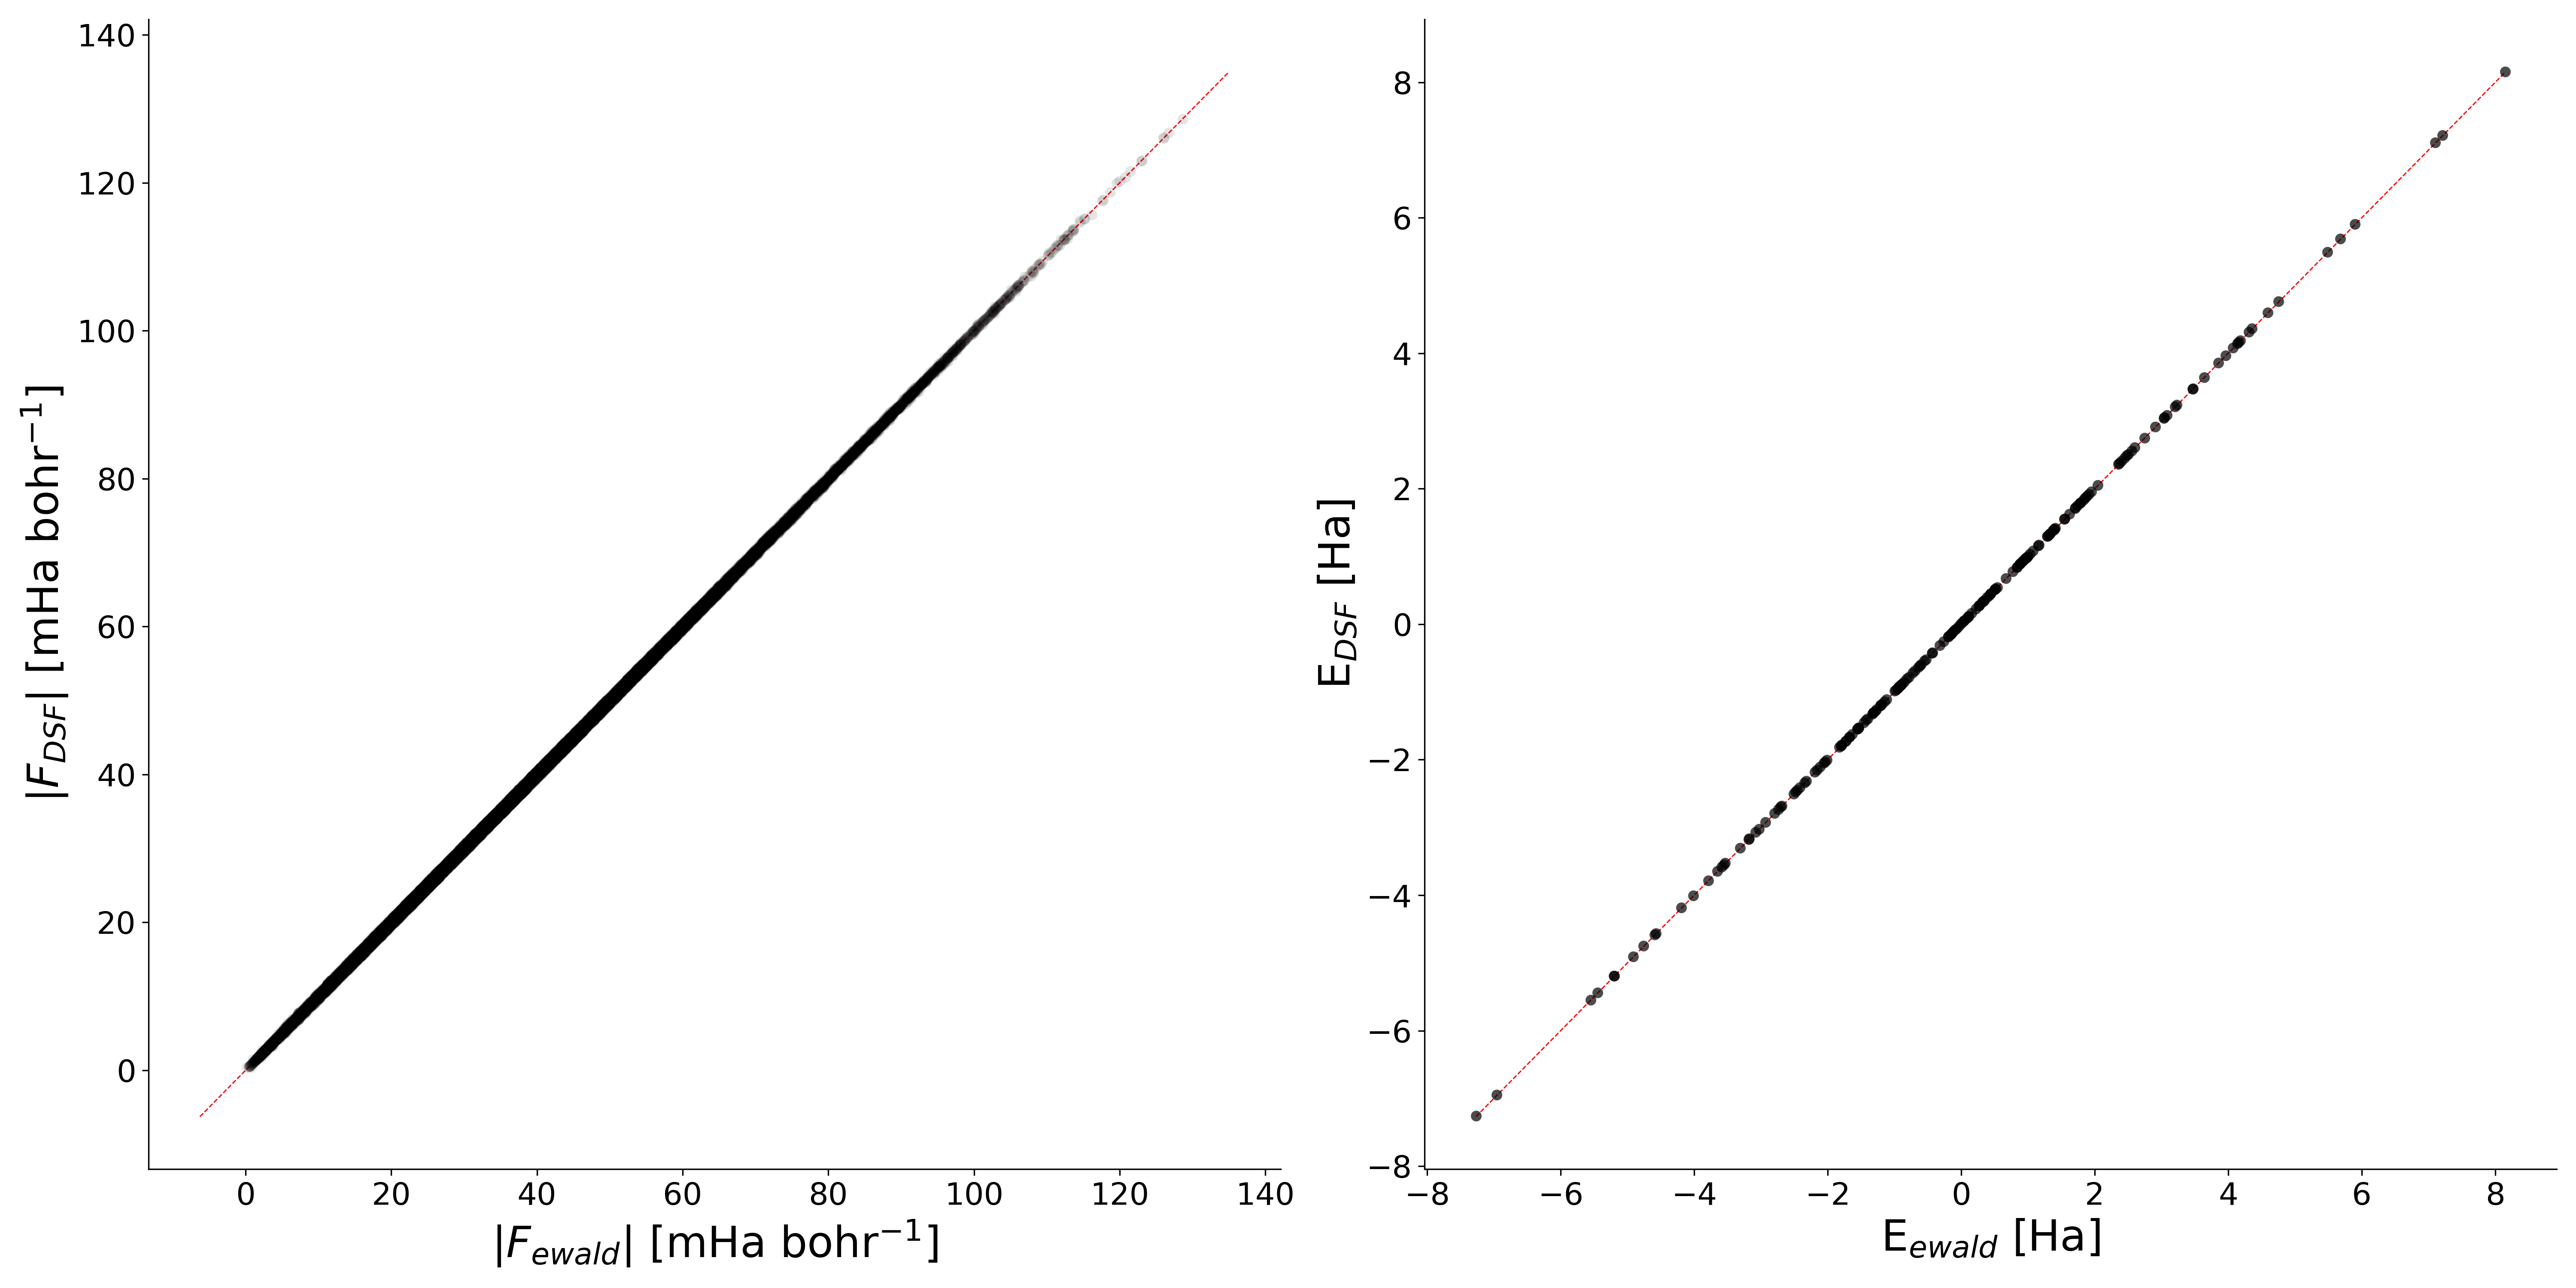
\includegraphics[width=\textwidth]{../img/ES/Ewald_DSF_Classical.png}
  \caption{\label{fig:Classical_DSF_Ewald}Comparison of Ewald and DSF forces and energies. The x-axis shows results from Ewald simulations and the y-axis shows results from DSF simulations. The left pane shows the force magnitude with black dots representing values from all atoms at all timesteps. The right pane shows potential energies from each timestep. The red line shows the line y=x and is a guide for the eye.}
\end{figure}
\\
In order to carry out a comparison to Ewald electrostatics, a small pentacene crystal was constructed, containing one hundred and twenty eight molecules. The standard triclinic pentacene unit cell was taken from the Cambridge Structural Database \cite{CSD} and the same forcefield parameters were used as in section \ref{chap:surface_hopping_app}. All molecules were in their neutral state (without an excess charge carrier). A 1ps classical molecular dynamics simulation was then performed with full Ewald electrostatics and positions and velocities were printed every 5fs. Two hundred separate simulations using DSF electrostatics were then performed using the printed geometries from the Ewald simulations. In these simulations an alpha of 0.0 and cutoff radius of twelve Angstrom was used. These were chosen as in Fennel, 06 \cite{DSF} as these values gave good results when compared to Ewald electrostatics. It is important to note that in this work the effect of the cutoff radius and the damping coefficient, $\alpha$, have not been investigated. The outputted energies and forces were subsequently compared and the RMSE was found for the difference between the Ewald and DSF simulations. Care was taken to shift both the Ewald and DSF energies by their mean value to correct for a different energy offset in their values. In order to put this RMSD in context, a further simulation was carried out without any electrostatic interactions on the outputted Ewald geometries. The energies and forces of this simulation were then subtracted from the Ewald energies and forces to isolate just the electrostatic interactions. The root mean squared fluctuations (RMSF) of just the electrostatic energies and forces were then calculated in order to quantify the error that DSF introduces. The root mean squared fluctuations of the Ewald electrostatic energies were calculated to be: 120.0 mHa and the root mean squared error in the DSF potential compared to the Ewald potential was calculated to be: 9.49 mHa. The root mean squared fluctuations of the Ewald electrostatic forces were calculated to be: 1.44 mHa bohr$^{-1}$ and the root mean squared error of DSF forces compared to Ewald forces were calculated to be: 0.13 mHa bohr$^{-1}$. These results show my implementation of DSF within CP2K to introduce an error of approximately eight to ten percent within the energies and forces. Further, we see in figure \ref{fig:Classical_DSF_Ewald} the magnitude of each Ewald and DSF force and each energy compared directly. When the coefficient of determination, R$^2$, is calculated for these data sets we get: 1.000 for the energies and forces, very similar values to the ones reported in Fennel, 06.
\\\\
As a final check of the equations the damping coefficient was set to a very large value (ten thousand) and each DSF interaction between pairs of atoms was printed. This was to confirm that, in the limit of an infinite $\alpha$ coefficient, DSF electrostatic contributions to the energies and forces tended to zero. 
\subsection{Surface Hopping}
Although, in surface hopping, the DSF equations are exactly the same the way that they are applied is quite different (as explained in \ref{sect:addSubMethod}). In order to test the DSF implementation in the surface hopping code the same two tests were run as in the classical code. The first was to compare each force and site-energy calculated using DSF with the addition-subtraction method to forces and site-energies calculated with N$_{mol}$ different topology files. The second was to compare the surface hopping DSF implementation with the already tested surface-hopping Ewald implementation.

\subsubsection{Multiple Topology Files}
\begin{figure}[ht]
  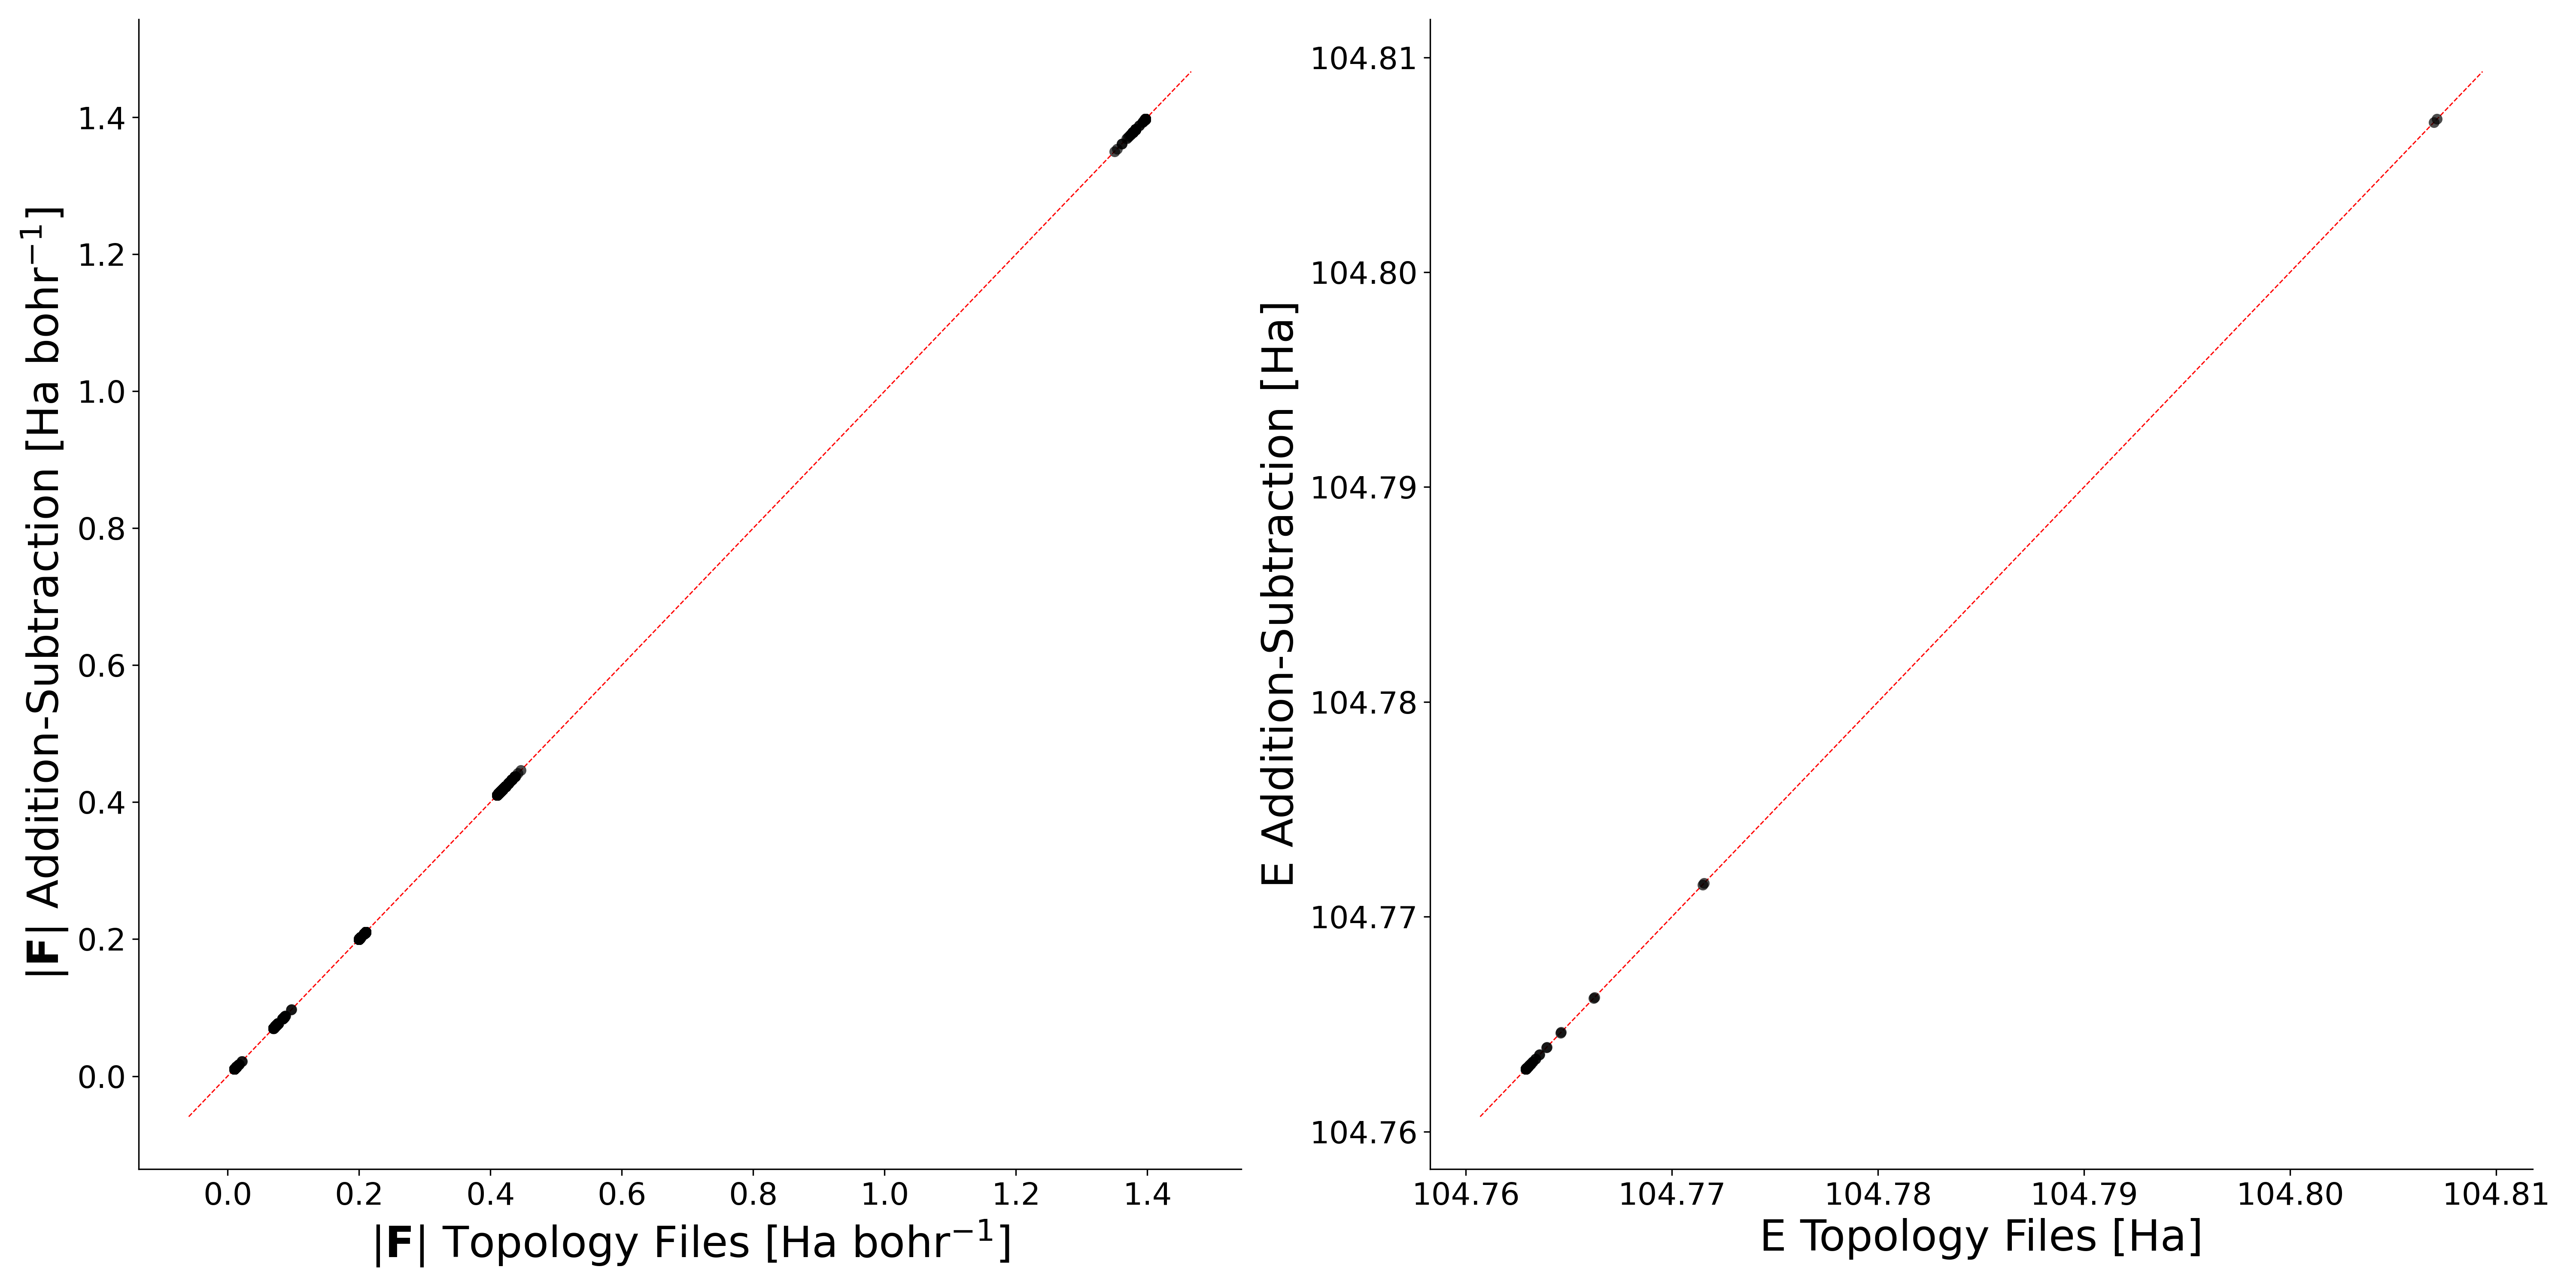
\includegraphics[width=\textwidth]{../img/ES/DSF_SH_test_topologies.png}
	\caption{\label{fig:FSSH_DSF_top}Comparison of DSF forces and energies using multiple topology files (x axis) and classical MD and using the addition-subtraction scheme within SH (y axis). The left pane shows the force magnitude with black dots representing values from all atoms at all timesteps. The right pane shows potential energies from each timestep. The red line shows the line y=x and serves as a guide for the eye.}
\end{figure}
\noindent As in section \ref{sect:testESimp}, the site-energies and forces for each permutation of the charged molecule were calculated by running N CP2K simulations. In each simulation, the inputted topology had a different molecule in the charged state and all the others in the neutral state. A one hundred molecule ethylene system was used and one hundred different simulations were run to get each site-energy and force (using DSF electrostatics). The forces and energies were outputted and used to compare to the forces and energies outputted from the surface hopping simulation using the addition subtraction scheme with DSF electrostatics. The results can be seen in figure \ref{fig:FSSH_DSF_top}. The maximum absolute difference in the outputted values was less than 10$^{-13}$ confirming the implementation of DSF with the addition-subtraction scheme in surface hopping.
\subsubsection{Comparison to Ewald}
\begin{figure}[htp]
  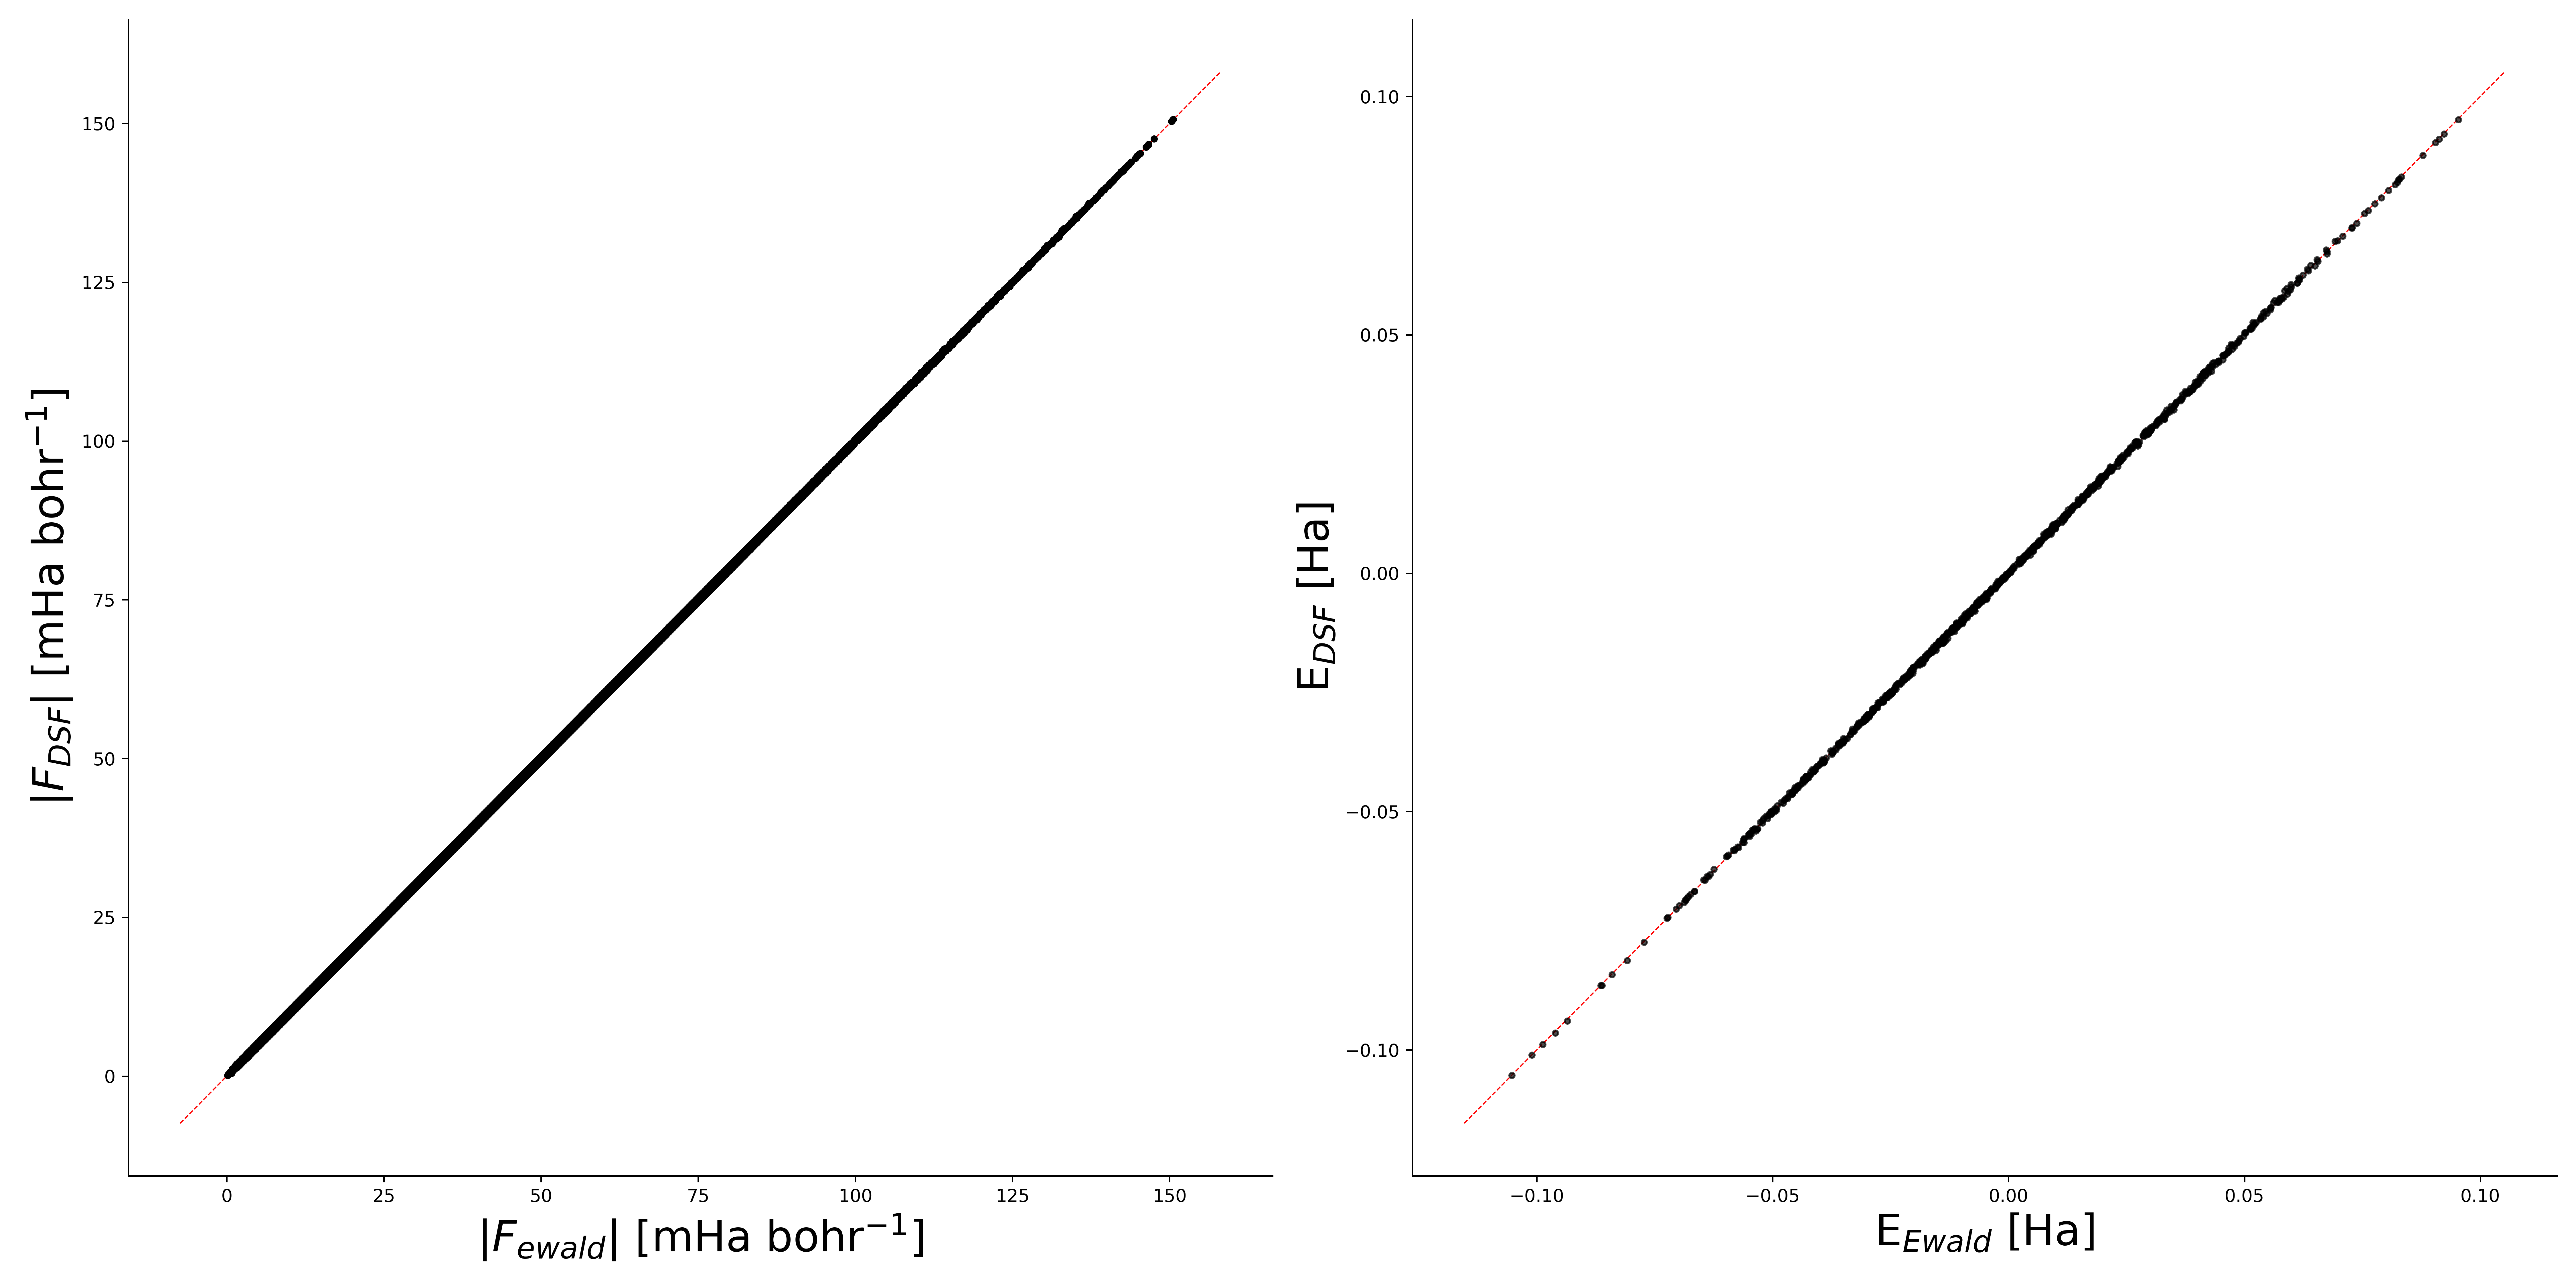
\includegraphics[width=\textwidth]{../img/ES/DSF_vs_Ewald_FSSH.png}
  \caption{\label{fig:DSF_vs_EwaldSH}A comparison of energies and forces as calculated by full Ewald and DSF electrostatics.}
\end{figure}
The comparison to Ewald electrostatics was carried out as in \ref{sect:ClassicalMDEwald}. That is, a surface hopping simulation was carried out with a small pentacene crystal and Ewald electrostatics. Positions and velocities were printed out periodically and DSF electrostatics was then run using each of the position and velocity files as initial geometries. A cutoff radius of fifteen Angstrom and damping coefficient of 0.0$bohr^{-1}$ was used. Forces and energies were then compared and the root mean squared deviation between Ewald and DSF was calculated. The system was a fifty four molecule pentacene crystal that had been equilibrated with classical MD using SPME as the electrostatic calculator, until the temperature and total energy had converged. The results are shown in figure \ref{fig:DSF_vs_EwaldSH}. 
\\\\
The results, reflect very well the findings from figure \ref{fig:Classical_DSF_Ewald}. This is to be expected as the same equations are being used. We see in both the forces and the energies that there is very little deviation of values with respect to full Ewald simulations at every timestep. In fact, the $R^2$ value is 1.000 for both datasets. As before the RMSF of the electrostatic energies and forces were calculated. These are 5.61 mHa and 0.60 mHa bohr$^{-1}$. The RMSE in the DSF electrostatics (compared to Ewald) was: 0.31 mHa and 0.08 mHa bohr$^{-1}$ for the total potential energy and forces respectively. This validates my implementation of DSF within surface hopping against my implementation of Ewald electrostatics. Further the Ewald implementation has been validated against classical MD and has been shown to reproduce the energies and forces exactly. Satisfied that the DSF implementation is working, in the following section, I will briefly show the speed up achieved by using DSF instead of Ewald electrostatics before final concluding remarks.

\section{Timing DSF}
\begin{figure}[htp]
  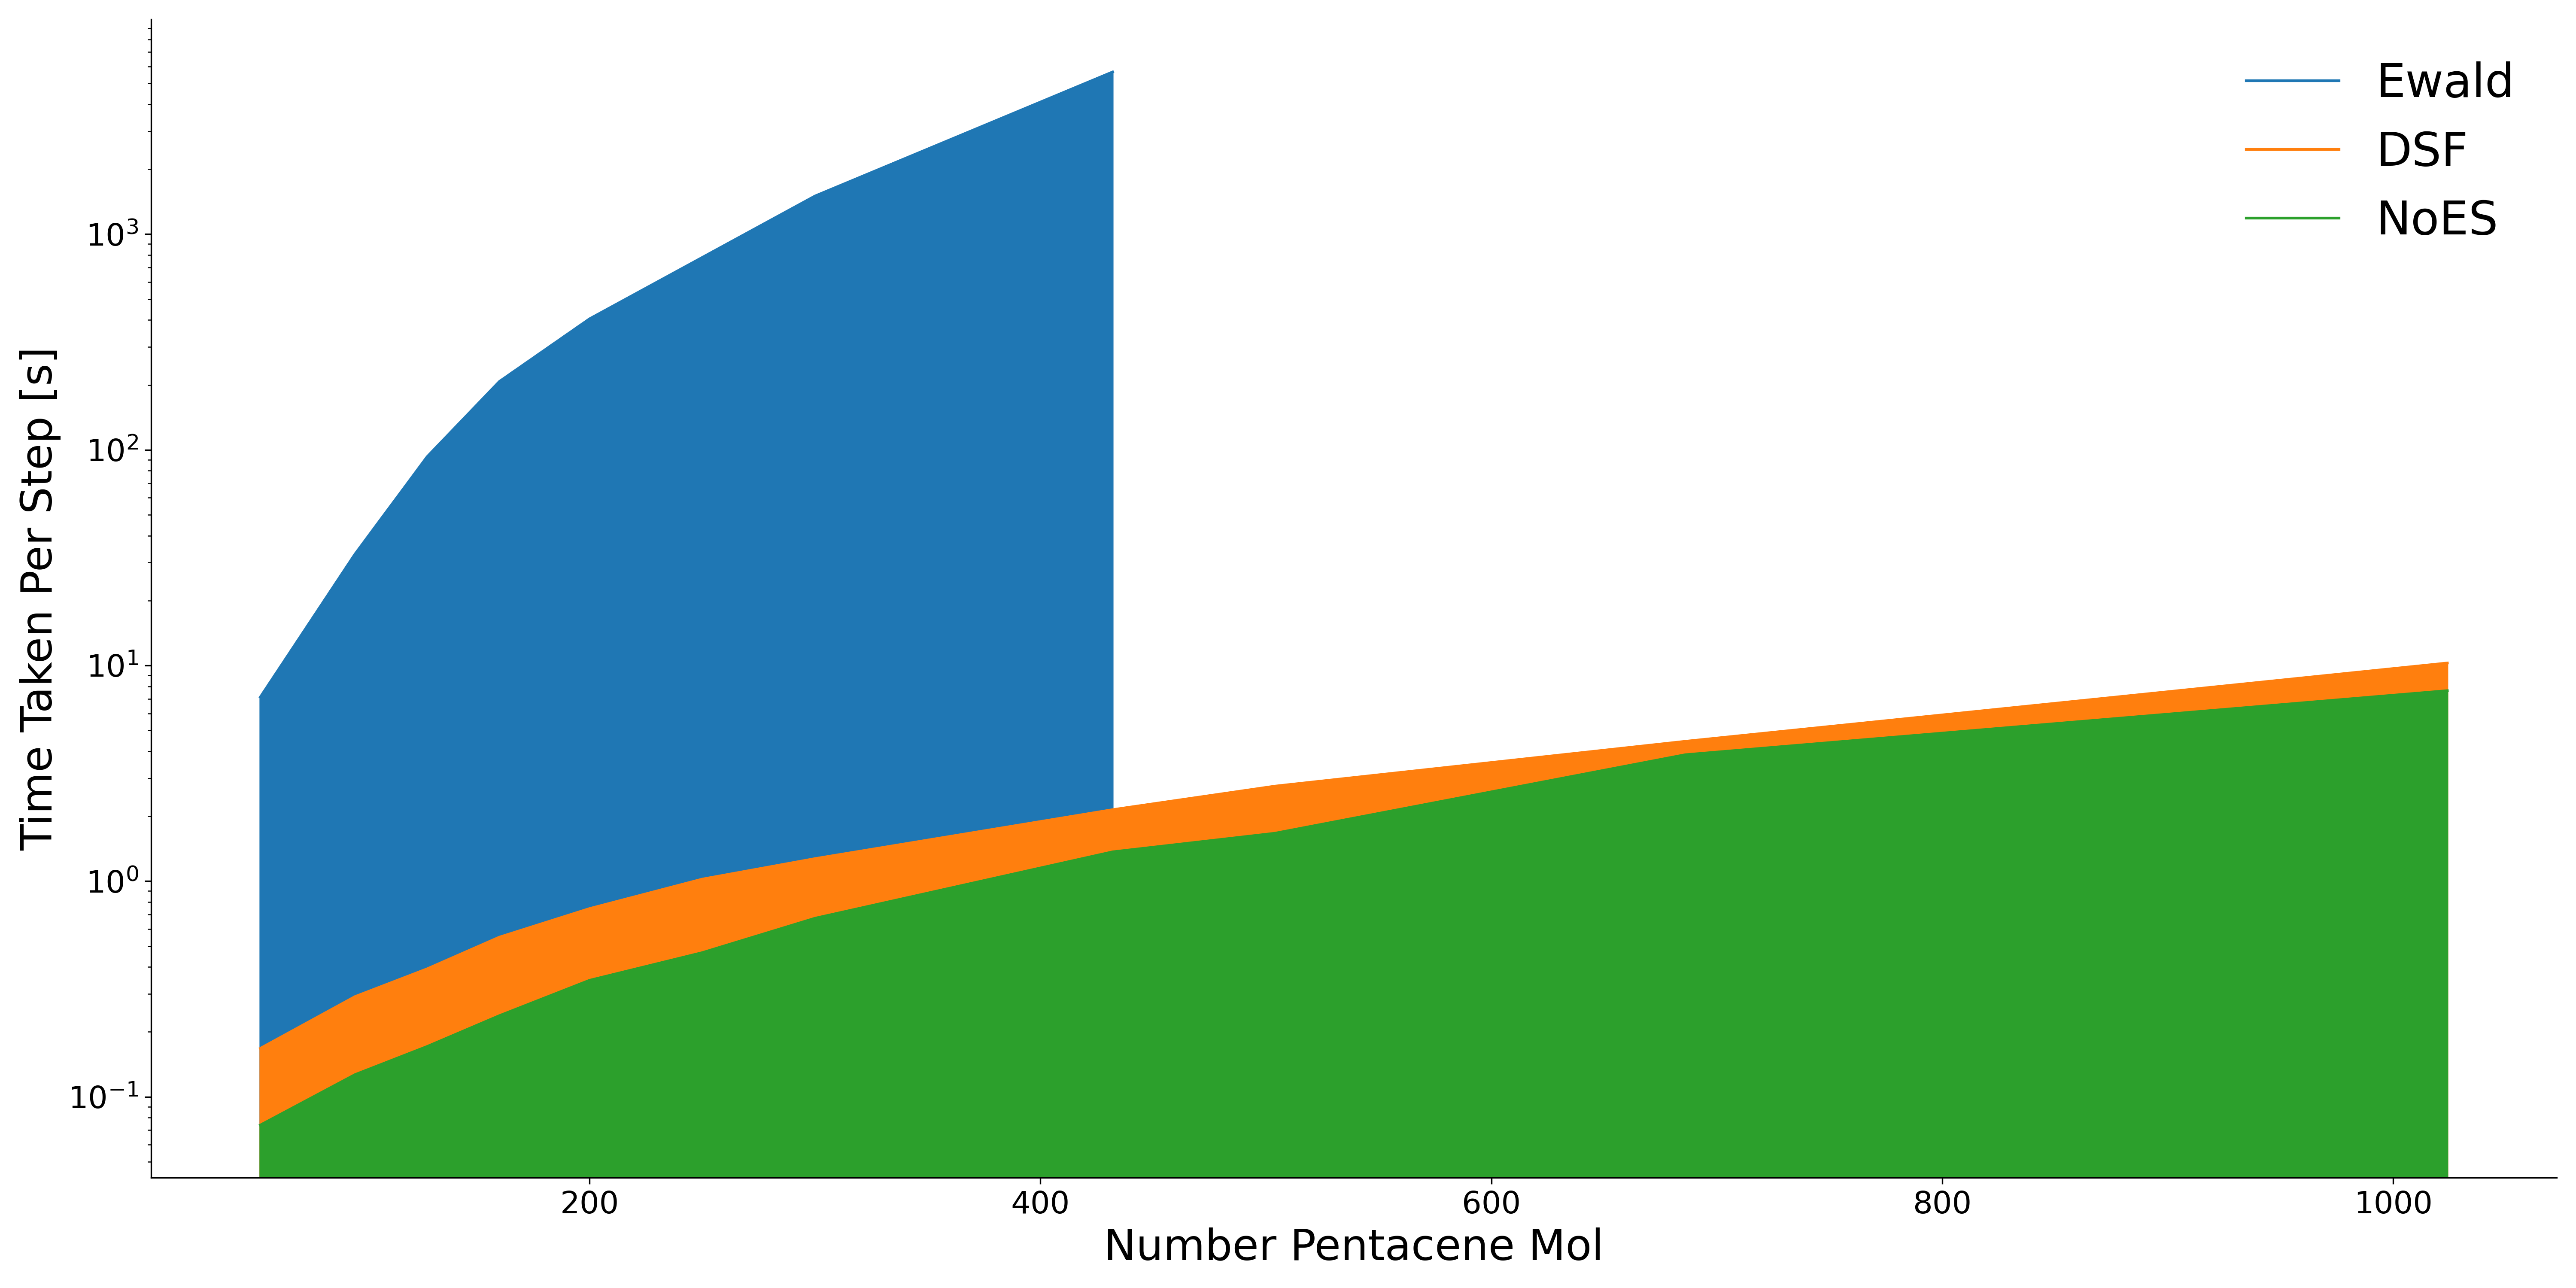
\includegraphics[width=\textwidth]{../img/ES/SH_timing_wEwald.png}
  \caption{\label{fig:DSF_Timings}Timing data on the DSF implementation compared to Ewald electrostatics and FOB-SH without any electrostatics. The blue curve shows Ewald timing data, the orange is DSF and green is without any electrostatics.}
\end{figure}
\noindent The DSF technique has been shown to give values for electrostatic energies and forces that very closely resemble Ewald electrostatics. However, if it does not provide a speedup to the code it has no use. In order to quantify the difference in time taken to calculate electrostatic interactions, I have ran a variety of simulations using Ewald electrostatics and DSF electrostatics in surface hopping and shown the results in figure \ref{fig:DSF_Timings}. In this figure we can clearly see that the DSF electrostatics results in a significant speedup of the Ewald code. At approximately fifty molecules calculating Ewald electrostatics (even with the addition-subtraction scheme) takes ten seconds per step. This would take approximately 2.3 days to simulate 1 ps, assuming a standard timestep of 0.05fs. This is because the reciprocal forces (forces calculated in reciprocal space in the Ewald sum) cannot be optimised with the addition-subtraction scheme. In contrast, if using DSF a single step would take around 0.08s and simulating 1ps would take less than thirty minutes. The filled orange shape shows the overhead that just the electrostatic calculations introduce compared to without electrostatics. The filled blue shape shows (slightly less than) the overhead that Ewald electrostatics introduces. We see in larger systems, such as the four hundred and thirty two molecule system calculating the electrostatic interactions alone takes more than one hour per step, the rest of the surface hopping code only requires around one second. This figure shows that using DSF electrostatics (with the addition-subtraction scheme) will allow simulation of around one thousand molecules in a reasonable time-frame.


%\section{Miscellaneous Optimisations}
%To help prepare the code for the study of larger systems, other group members and I implemented various other 

\section{Conclusions}
In this chapter I have presented an extension to the surface hopping code, namely the implementation of electrostatic interactions. I have tested and timed my implementation of the standard Ewald summation technique and the damped shifted forces (DSF) method. I have discussed the limitations in the standard Ewald technique, i.e. far too costly for large systems and discussed how these can be mitigated with the DSF method. Due to the way the Hamiltonian is constructed in FOB-SH, each diagonal element (site-energy) is calculated by calculating all forces and energies. There are $N_{mol}$ site-energies leading to a scaling in CPU time of $O(N_{mol} N_{atom}^2)$. However, the use of an addition-subtraction scheme has been shown to successfully reduce this by an order of magnitude ($N_{mol}$), allowing the simulation of large systems requiring the proper account of electrostatic interactions (such as polar systems or highly disordered ones). However, this addition-subtraction scheme cannot be applied to the reciprocal space forces in the Ewald summation. For this reason, DSF has been implemented to provide a reasonable estimate of full Ewald forces and energies. In the systems tested in this chapter the error produced by DSF was around eight to ten percent compared with Ewald electrostatics. Although with appropriate tuning of input parameters this may be reduced even further. An investigation of the parameters has not been carried out in this work due to time constraints, though should be a relatively straightforward task. Importantly, the use of the DSF technique in calculating electrostatic interactions has been shown to add very little overhead to the bare surface hopping code. Using a one thousand and twenty four molecule pentacene system the time taken per step increases from 7.5 seconds to 10.5 seconds without and with DSF electrostatics respectively.
\\\\
The results in this chapter report a very promising start to the generalisation of the FOB-SH code to systems requiring electrostatic interactions. However, more work should be done to further test both the effect of parameters $\alpha$ and $R_{cut}$, and to compare outputted physical properties such as electronic populations and system structure to a reference system. This could mean simulating small three dimensional structures with both Ewald electrostatics and DSF and comparing structures and mobilities. Further, it would be interesting to apply the DSF enabled FOB-SH code to the amorphous and crystalline structures from the previous chapter and to observe their effect on charge trapping -especially in interfacial regions.

